\documentclass{article}
\usepackage{graphicx} 
\usepackage[a4paper, total={6in, 8in}]{geometry}
\usepackage{caption}
\usepackage{subcaption}

\title{Performance Report}
\author{Ruhul Azgor}
\date{\today}

\begin{document}

\maketitle

\section{Learning Curve of Different Model}
For all the models, the given parameter was set.
\begin{itemize}
    \item Mini-batch size: 1024
    \item Learning Rate decay: 0.5
    \item Beta1: 0.9
    \item Beta2: 0.99
    \item Epsilon: 1e-8
    \item Xavier Initialization
\end{itemize}
\subsection{Model 1}
\subsubsection{Architecture}
\begin{verbatim}
    Dense(784, 512),
    Relu(),
    Dropout(probability=.15),
    Dense(512, 256),
    Relu(),
    Dropout(probability=.15),
    Dense(256, 128),
    Relu(),
    Dropout(probability=.10),
    Dense(128, 64),
    Relu(),
    Dropout(probability=.10),
    Dense(64, 26),
    Softmax()
\end{verbatim}
\subsubsection{Learning Rate = 0.01}
Best Performance:
\begin{itemize}
    \item Best epoch: 50
    \item train loss: 0.2602
    \item validation loss: 0.2892
    \item train accuracy: 0.9142
    \item validation accuracy: 0.9099
    \item validation f1 score: 0.9096
\end{itemize}

\begin{figure}[h]
    \begin{subfigure}{0.5\textwidth}
        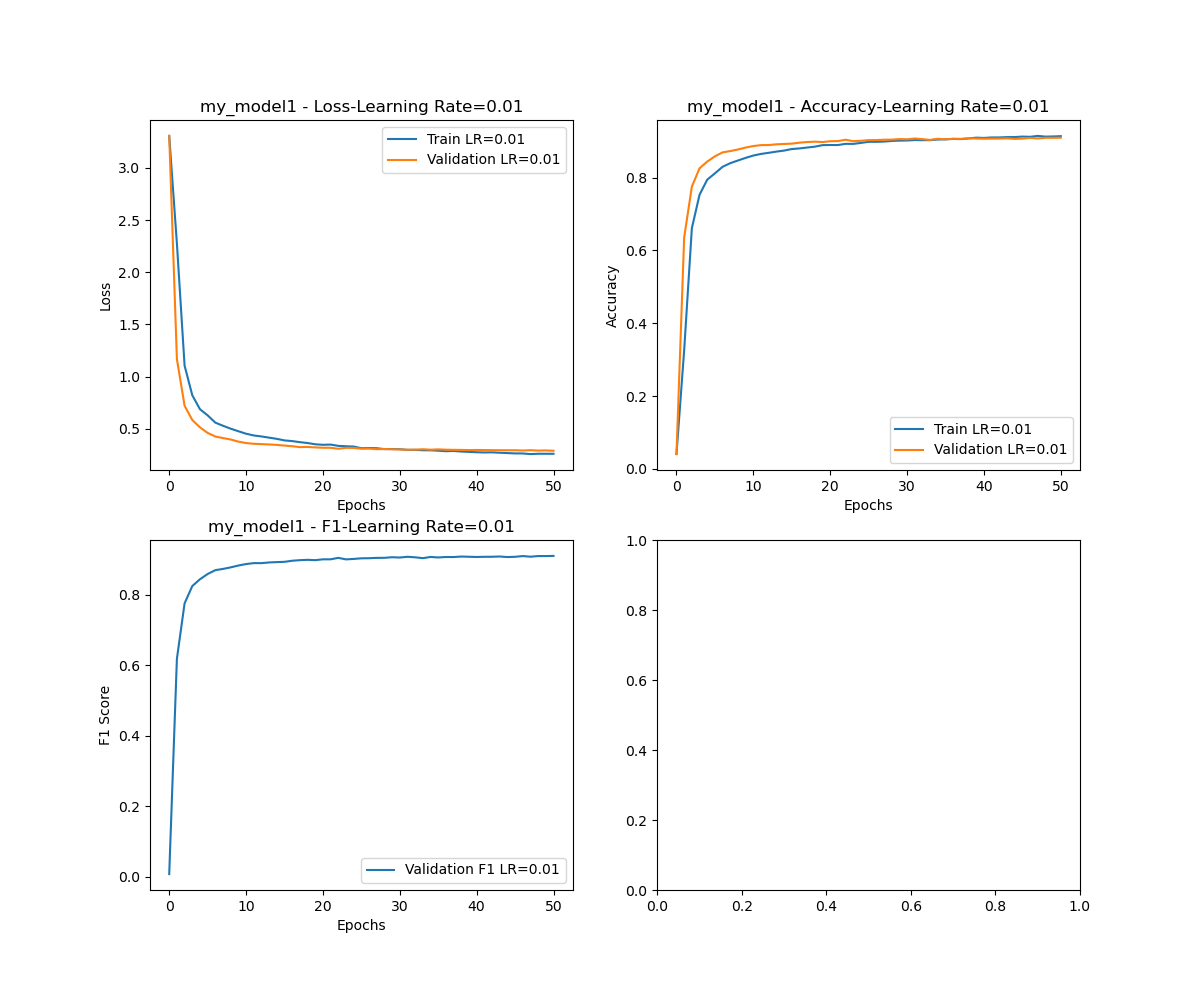
\includegraphics[width=\linewidth, height=6cm]{Images/my_model1_0.01.png} 
        \caption{Model 1 Learning Curve with Learning Rate 0.01}
        \label{fig:model1_lr_0.01}
    \end{subfigure}
    \begin{subfigure}{0.5\textwidth}
        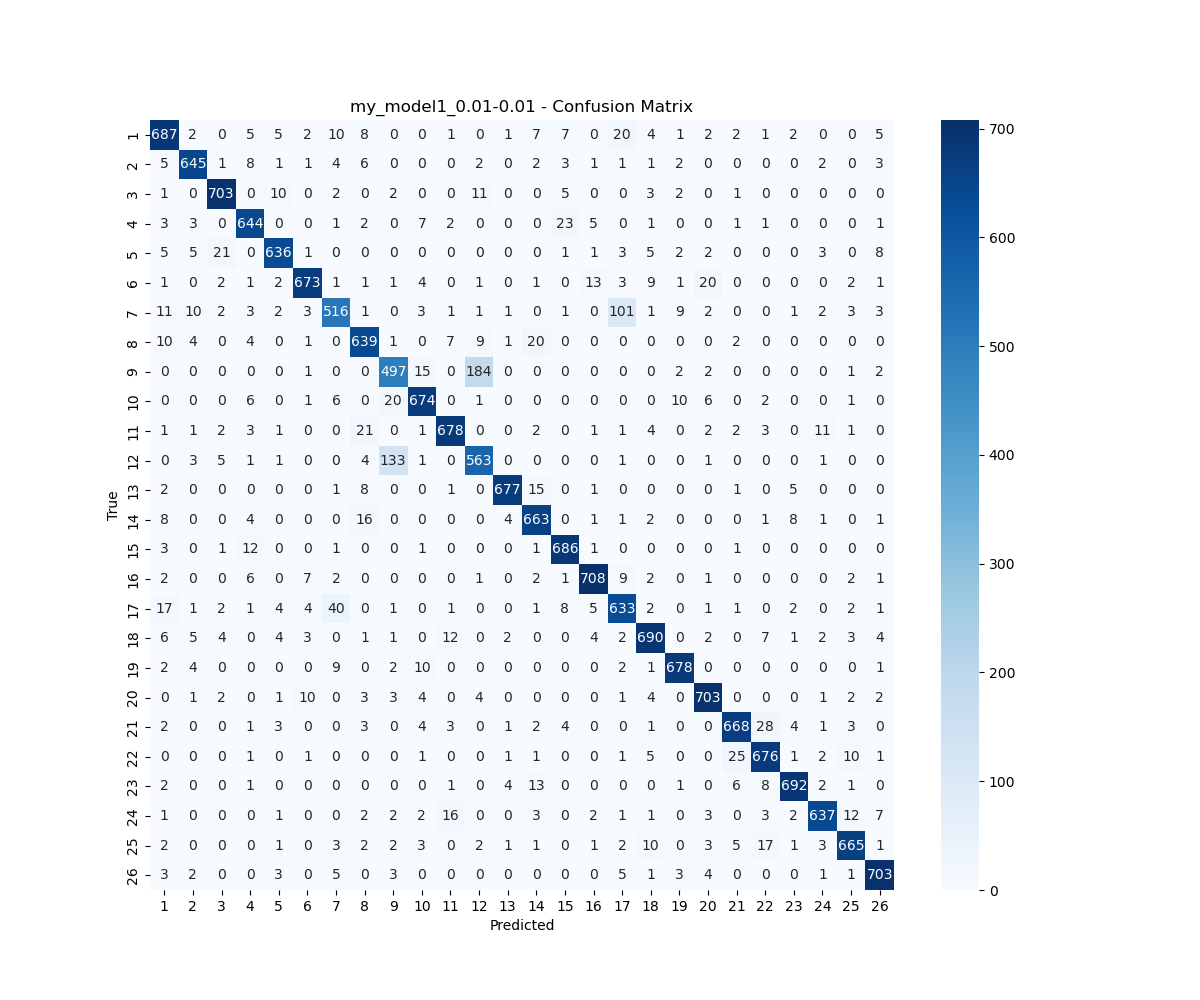
\includegraphics[width=\linewidth, height=6cm]{Images/my_model1_0.01-confusion_matrix} 
        \caption{Model 1 Confusion Matrix with Learning Rate 0.01}
        \label{fig:model1_lr_0.01_confusion_matrix}
    \end{subfigure}
    \caption{Model 1 Learning Curve and Confusion Matrix with Learning Rate 0.01}
    \label{fig:model1_lr_0.01_combined}
\end{figure}

\subsubsection{Learning Rate = 0.005}
Best Performance:
\begin{itemize}
    \item Best epoch: 50
    \item train loss: 0.1554
    \item validation loss: 0.2662
    \item train accuracy: 0.9448
    \item validation accuracy: 0.9206
    \item validation f1 score: 0.9204
\end{itemize}

\begin{figure}[h]
    \begin{subfigure}{0.5\textwidth}
        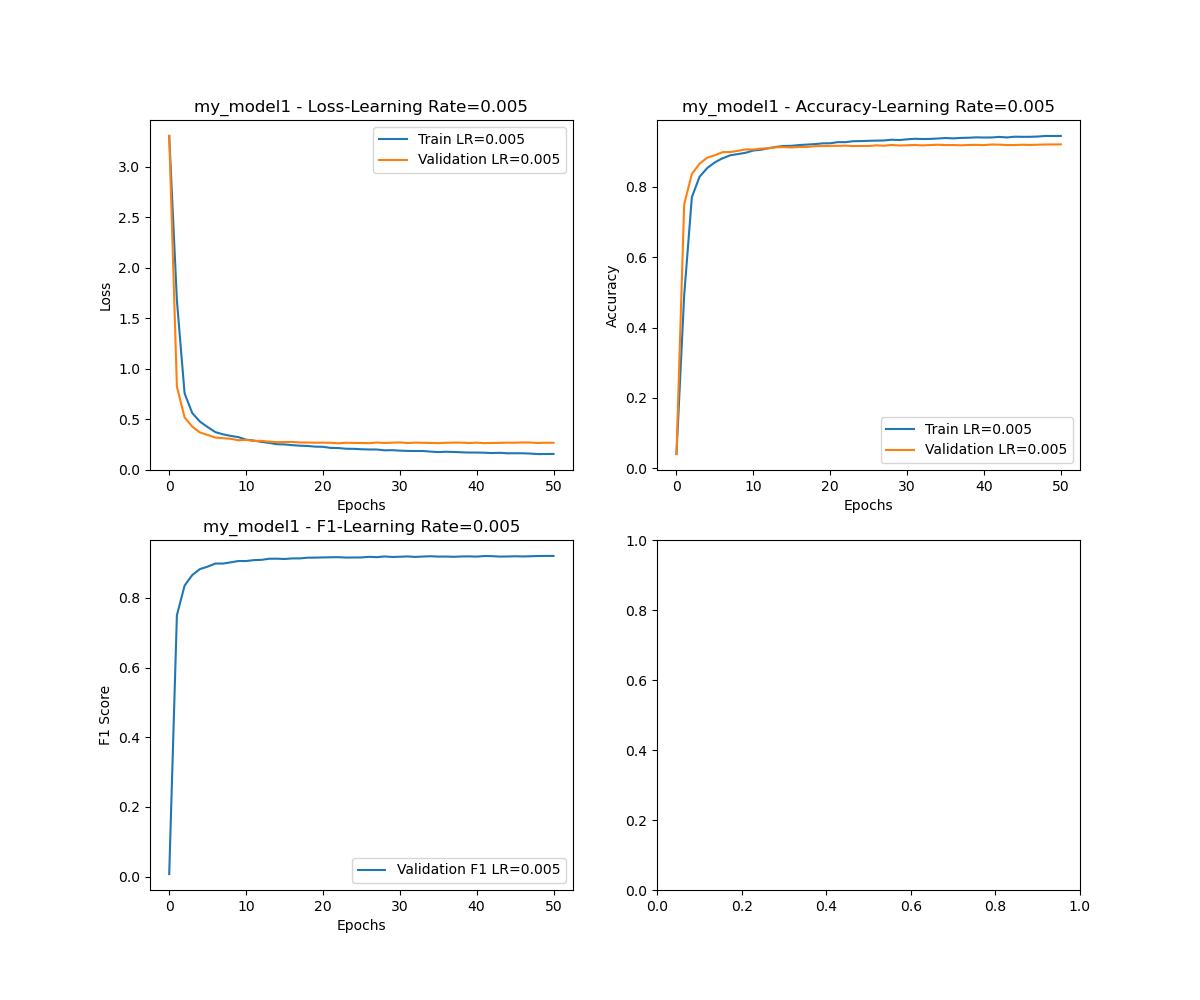
\includegraphics[width=\linewidth, height=6cm]{Images/my_model1_0.005.png} 
        \caption{Model 1 Learning Curve with Learning Rate 0.005}
        \label{fig:model1_lr_0.005}
    \end{subfigure}
    \begin{subfigure}{0.5\textwidth}
        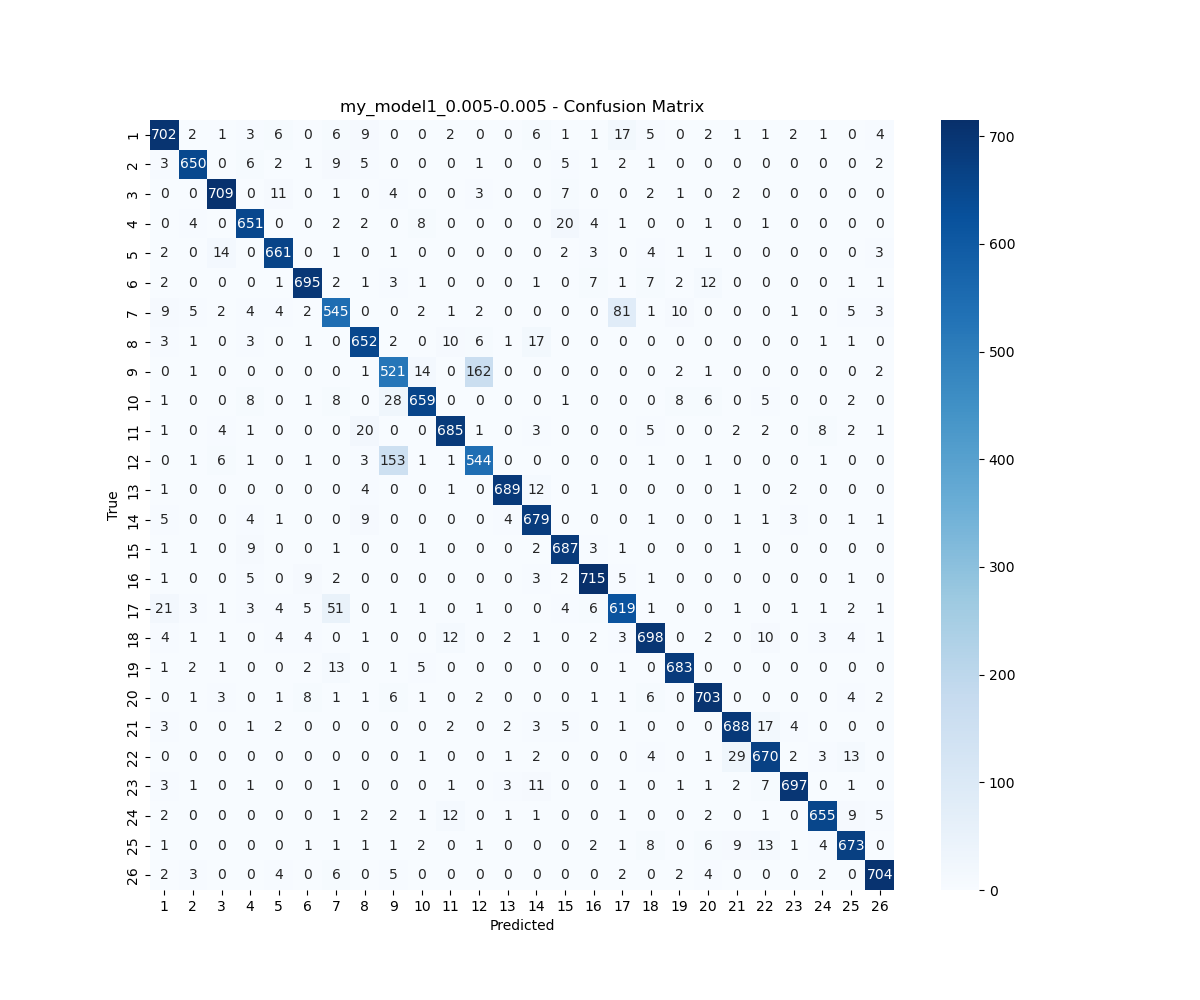
\includegraphics[width=\linewidth, height=6cm]{Images/my_model1_0.005-confusion_matrix} 
        \caption{Model 1 Confusion Matrix with Learning Rate 0.005}
        \label{fig:model1_lr_0.005_confusion_matrix}
    \end{subfigure}
    \caption{Model 1 Learning Curve and Confusion Matrix with Learning Rate 0.005}
    \label{fig:model1_lr_0.005_combined}
\end{figure}

\subsubsection{Learning Rate = 0.001}
Best Performance:
\begin{itemize}
    \item Best epoch: 49
    \item train loss: 0.2959
    \item validation loss: 0.2793
    \item train accuracy: 0.9046
    \item validation accuracy: 0.9105
    \item validation f1 score: 0.9102
\end{itemize}

\begin{figure}[h]
    \begin{subfigure}{0.5\textwidth}
        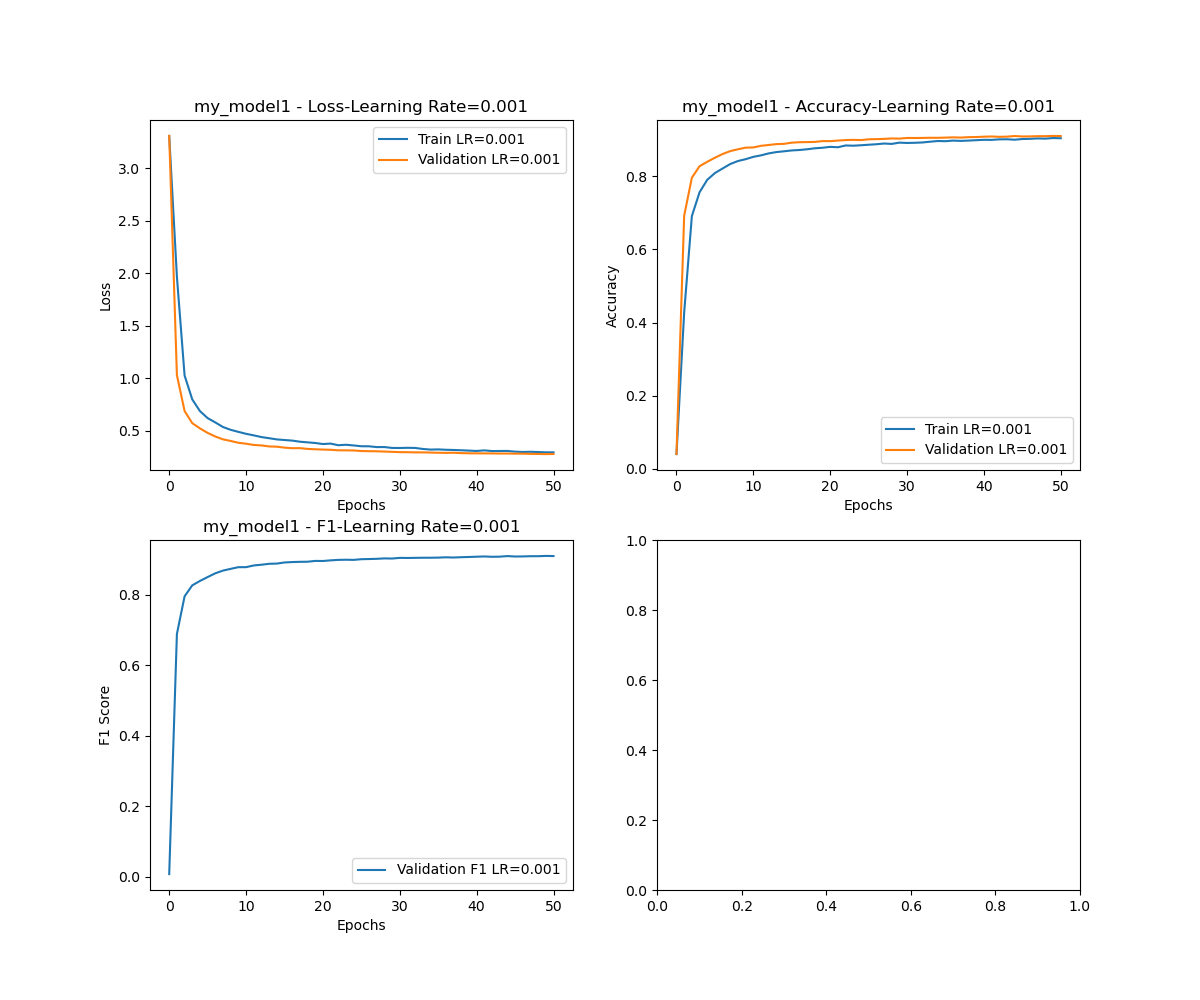
\includegraphics[width=\linewidth, height=6cm]{Images/my_model1_0.001.png} 
        \caption{Model 1 Learning Curve with Learning Rate 0.001}
        \label{fig:model1_lr_0.001}
    \end{subfigure}
    \begin{subfigure}{0.5\textwidth}
        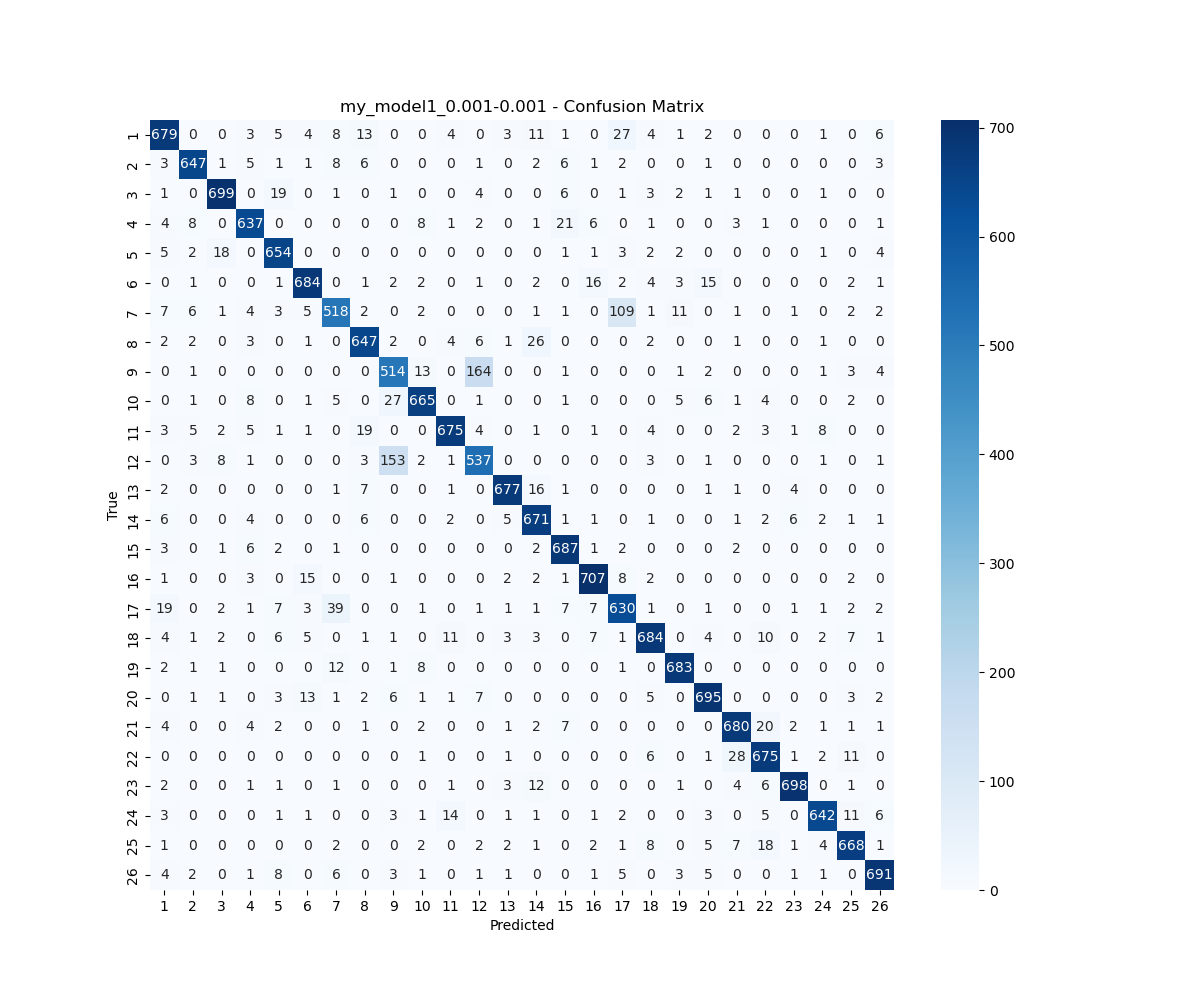
\includegraphics[width=\linewidth, height=6cm]{Images/my_model1_0.001-confusion_matrix} 
        \caption{Model 1 Confusion Matrix with Learning Rate 0.001}
        \label{fig:model1_lr_0.001_confusion_matrix}
    \end{subfigure}
    \caption{Model 1 Learning Curve and Confusion Matrix with Learning Rate 0.001}
    \label{fig:model1_lr_0.001_combined}
\end{figure}

\subsubsection{Learning Rate = 0.0005}
Best Performance:
\begin{itemize}
    \item Best epoch: 47
    \item train loss: 0.4765
    \item validation loss: 0.3790
    \item train accuracy: 0.8521
    \item validation accuracy: 0.8822
    \item validation f1 score: 0.8818
\end{itemize}

\begin{figure}[h]
    \begin{subfigure}{0.5\textwidth}
        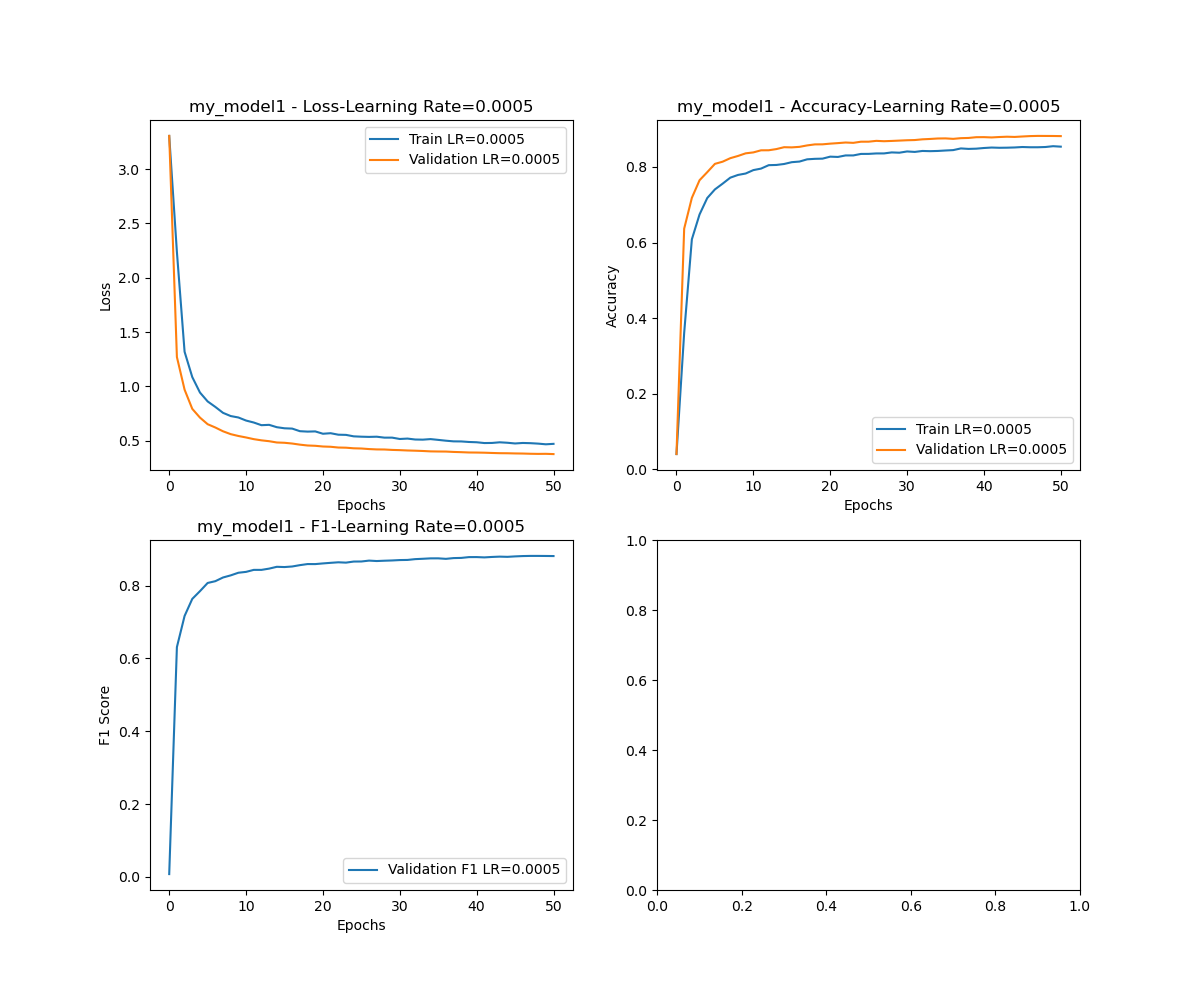
\includegraphics[width=\linewidth, height=6cm]{Images/my_model1_0.0005.png} 
        \caption{Model 1 Learning Curve with Learning Rate 0.0005}
        \label{fig:model1_lr_0.0005}
    \end{subfigure}
    \begin{subfigure}{0.5\textwidth}
        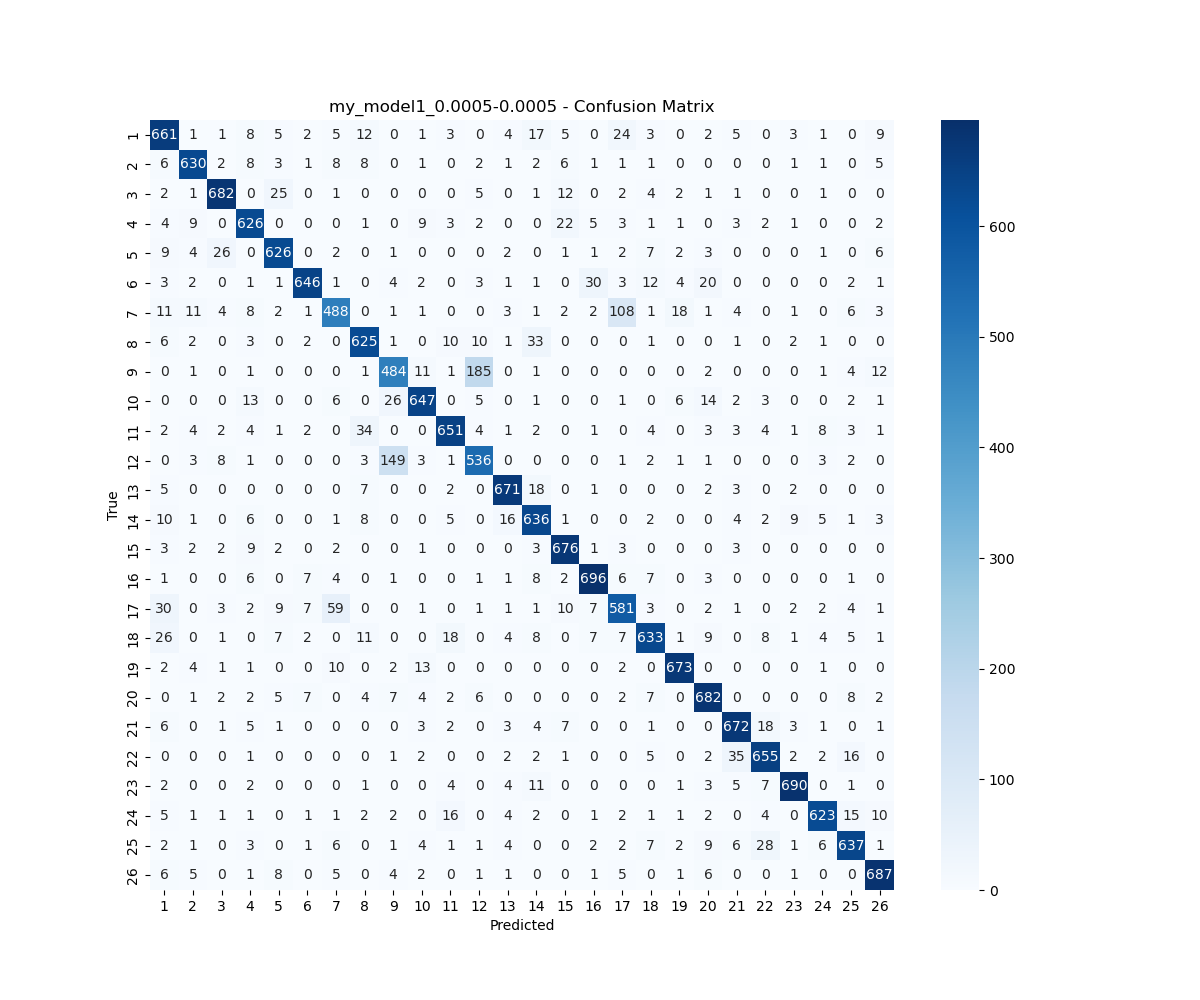
\includegraphics[width=\linewidth, height=6cm]{Images/my_model1_0.0005-confusion_matrix} 
        \caption{Model 1 Confusion Matrix with Learning Rate 0.0005}
        \label{fig:model1_lr_0.0005_confusion_matrix}
    \end{subfigure}
    \caption{Model 1 Learning Curve and Confusion Matrix with Learning Rate 0.0005}
    \label{fig:model1_lr_0.0005_combined}
\end{figure}

\subsection{Model 2}
\subsubsection{Architecture}
\begin{verbatim}
    Dense(784, 2048),
    Relu(),
    Dropout(probability=.4),
    Dense(2048, 1024),
    Relu(),
    Dropout(probability=.3),
    Dense(1024, 26),
    Softmax()
\end{verbatim}

\subsubsection{Learning Rate = 0.01}
% Best epoch: 47, validation accuracy: 0.9074, validation f1 score: 0.9073, model name: my_model2_0.01,
%           train loss: 0.3481, validation loss: 0.2996, train accuracy: 0.8846, validation accuracy: 0.9074
Best Performance:
\begin{itemize}
    \item Best epoch: 47
    \item train loss: 0.3481
    \item validation loss: 0.2996
    \item train accuracy: 0.8846
    \item validation accuracy: 0.9074
    \item validation f1 score: 0.9073
\end{itemize}

\begin{figure}[h]
    \begin{subfigure}{0.5\textwidth}
        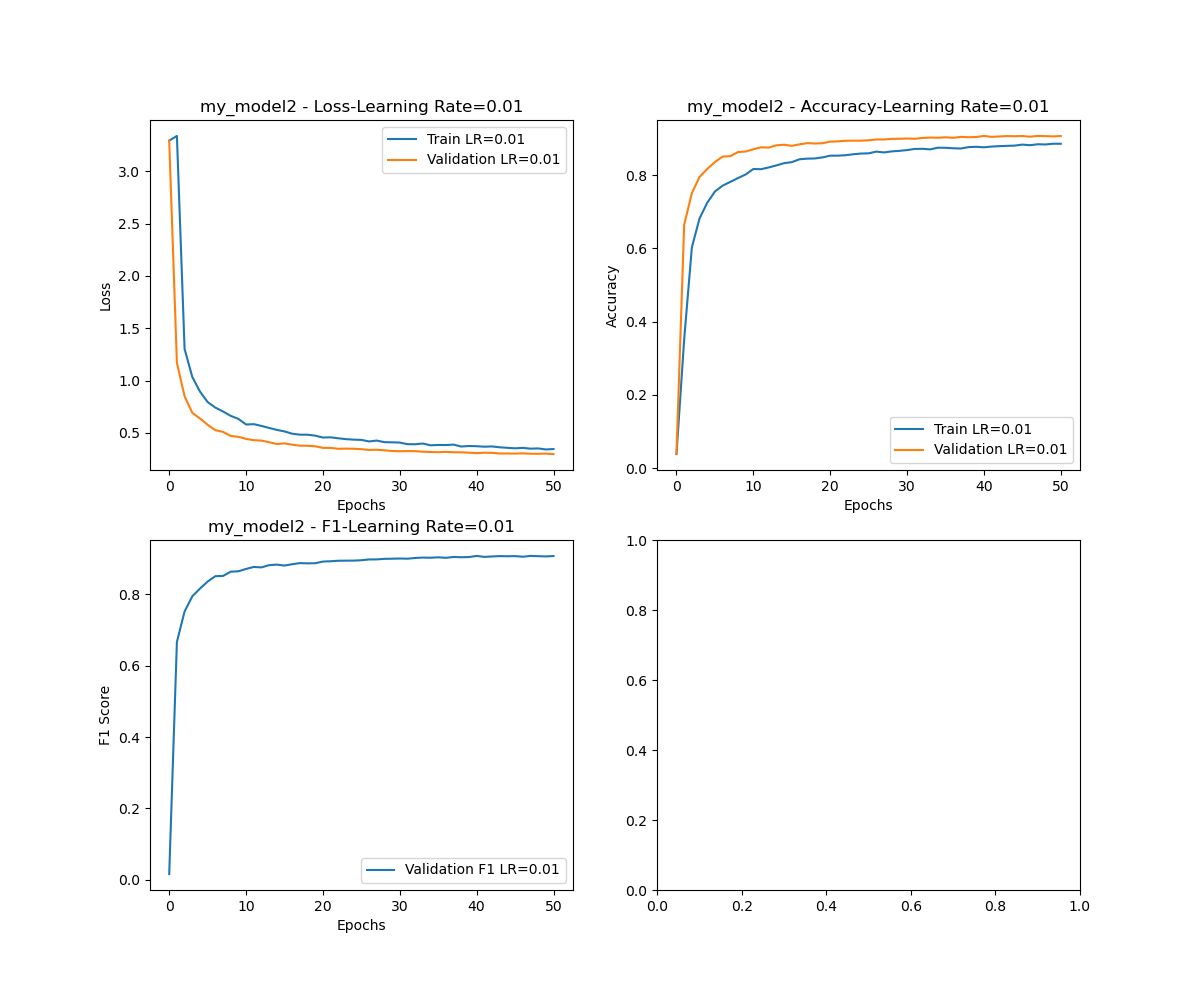
\includegraphics[width=\linewidth, height=6cm]{Images/my_model2_0.01.png} 
        \caption{Model 2 Learning Curve with Learning Rate 0.01}
        \label{fig:model2_lr_0.01}
    \end{subfigure}
    \begin{subfigure}{0.5\textwidth}
        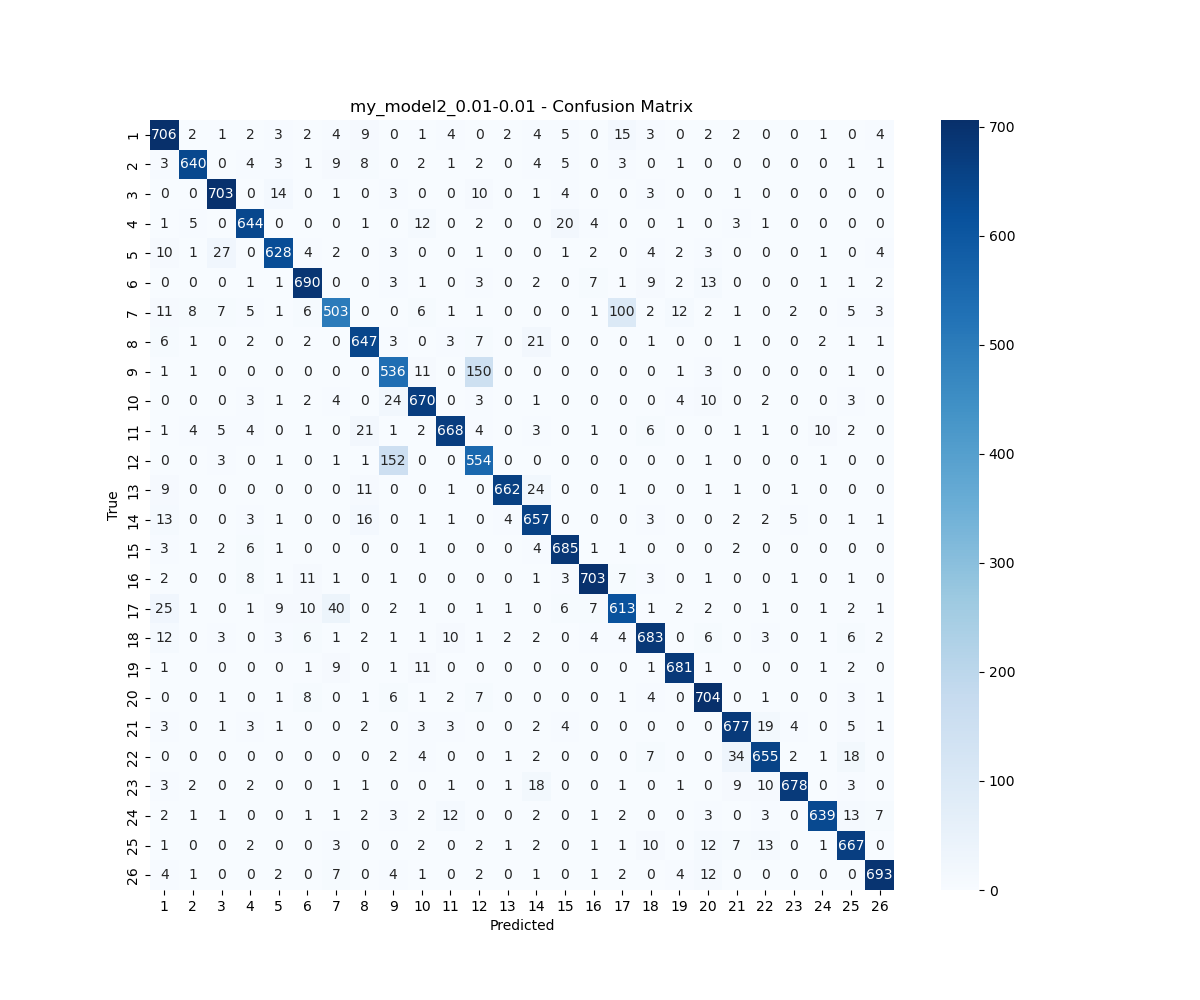
\includegraphics[width=\linewidth, height=6cm]{Images/my_model2_0.01-confusion_matrix} 
        \caption{Model 2 Confusion Matrix with Learning Rate 0.01}
        \label{fig:model2_lr_0.01_confusion_matrix}
    \end{subfigure}
    \caption{Model 2 Learning Curve and Confusion Matrix with Learning Rate 0.01}
    \label{fig:model2_lr_0.01_combined}
\end{figure}

\subsubsection{Learning Rate = 0.005}
% Best epoch: 49, validation accuracy: 0.9239, validation f1 score: 0.9237, model name: my_model2_0.005,
%           train loss: 0.1622, validation loss: 0.2358, train accuracy: 0.9413, validation accuracy: 0.9239
Best Performance:
\begin{itemize}
    \item Best epoch: 49
    \item train loss: 0.1622
    \item validation loss: 0.2358
    \item train accuracy: 0.9413
    \item validation accuracy: 0.9239
    \item validation f1 score: 0.9237
\end{itemize}

\begin{figure}[h]
    \begin{subfigure}{0.5\textwidth}
        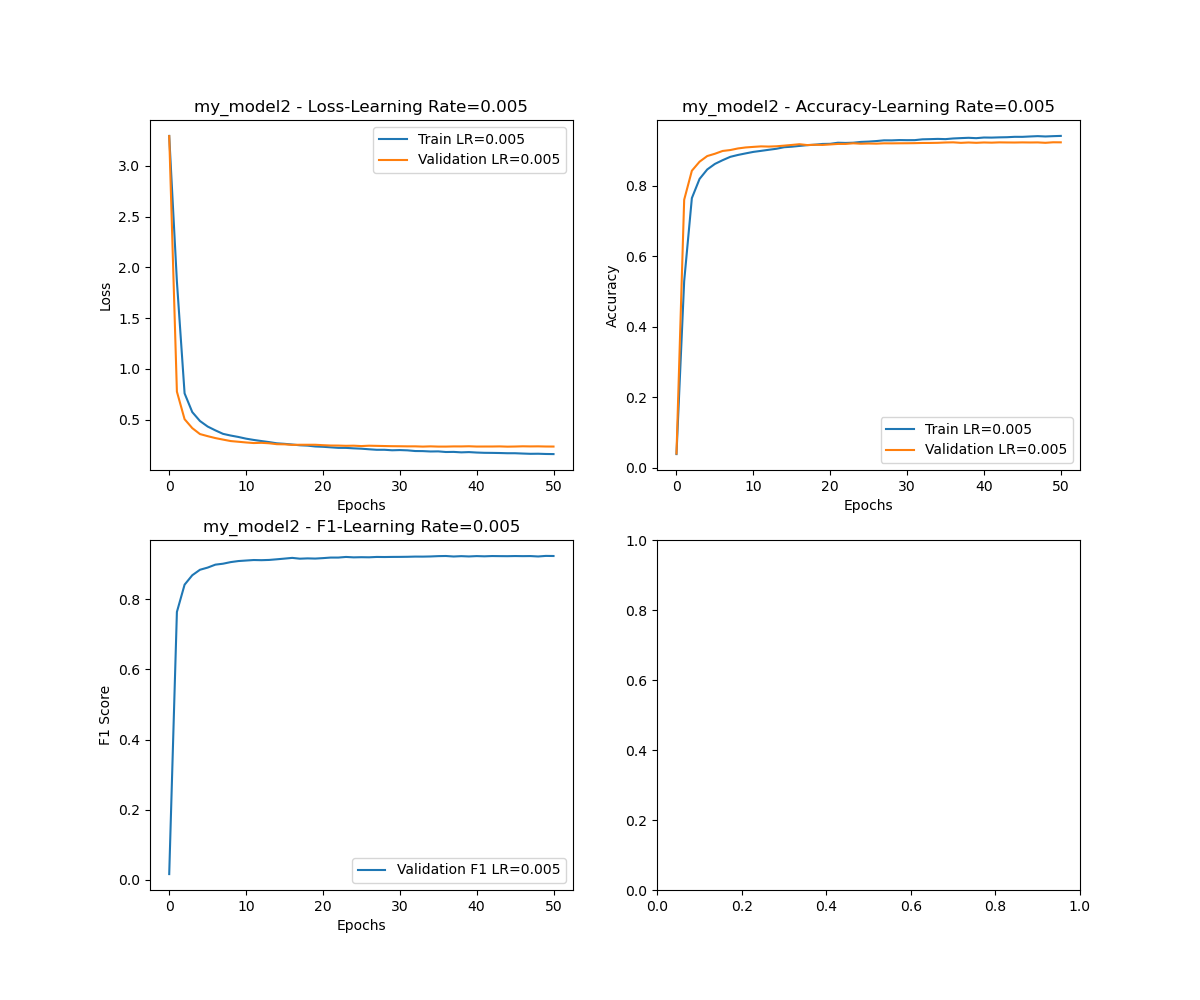
\includegraphics[width=\linewidth, height=6cm]{Images/my_model2_0.005.png} 
        \caption{Model 2 Learning Curve with Learning Rate 0.005}
        \label{fig:model2_lr_0.005}
    \end{subfigure}
    \begin{subfigure}{0.5\textwidth}
        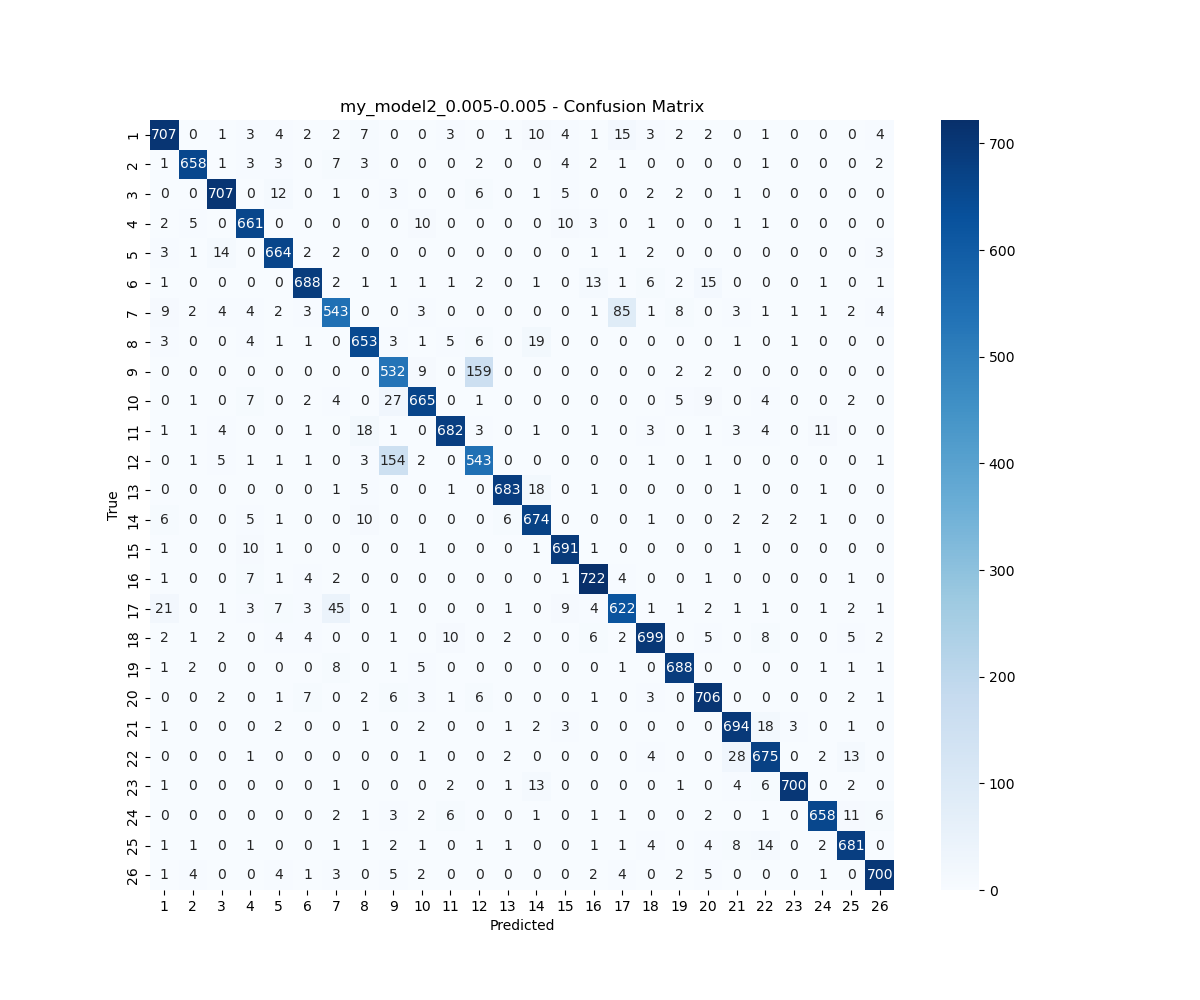
\includegraphics[width=\linewidth, height=6cm]{Images/my_model2_0.005-confusion_matrix} 
        \caption{Model 2 Confusion Matrix with Learning Rate 0.005}
        \label{fig:model2_lr_0.005_confusion_matrix}
    \end{subfigure}
    \caption{Model 2 Learning Curve and Confusion Matrix with Learning Rate 0.005}
    \label{fig:model2_lr_0.005_combined}
\end{figure}

\subsubsection{Learning Rate = 0.001}
% Best epoch: 49, validation accuracy: 0.9248, validation f1 score: 0.9246, model name: my_model2_0.001,
%           train loss: 0.1542, validation loss: 0.2268, train accuracy: 0.9467, validation accuracy: 0.9248
Best Performance:
\begin{itemize}
    \item Best epoch: 49
    \item train loss: 0.1542
    \item validation loss: 0.2268
    \item train accuracy: 0.9467
    \item validation accuracy: 0.9248
    \item validation f1 score: 0.9246
\end{itemize}

\begin{figure}[h]
    \begin{subfigure}{0.5\textwidth}
        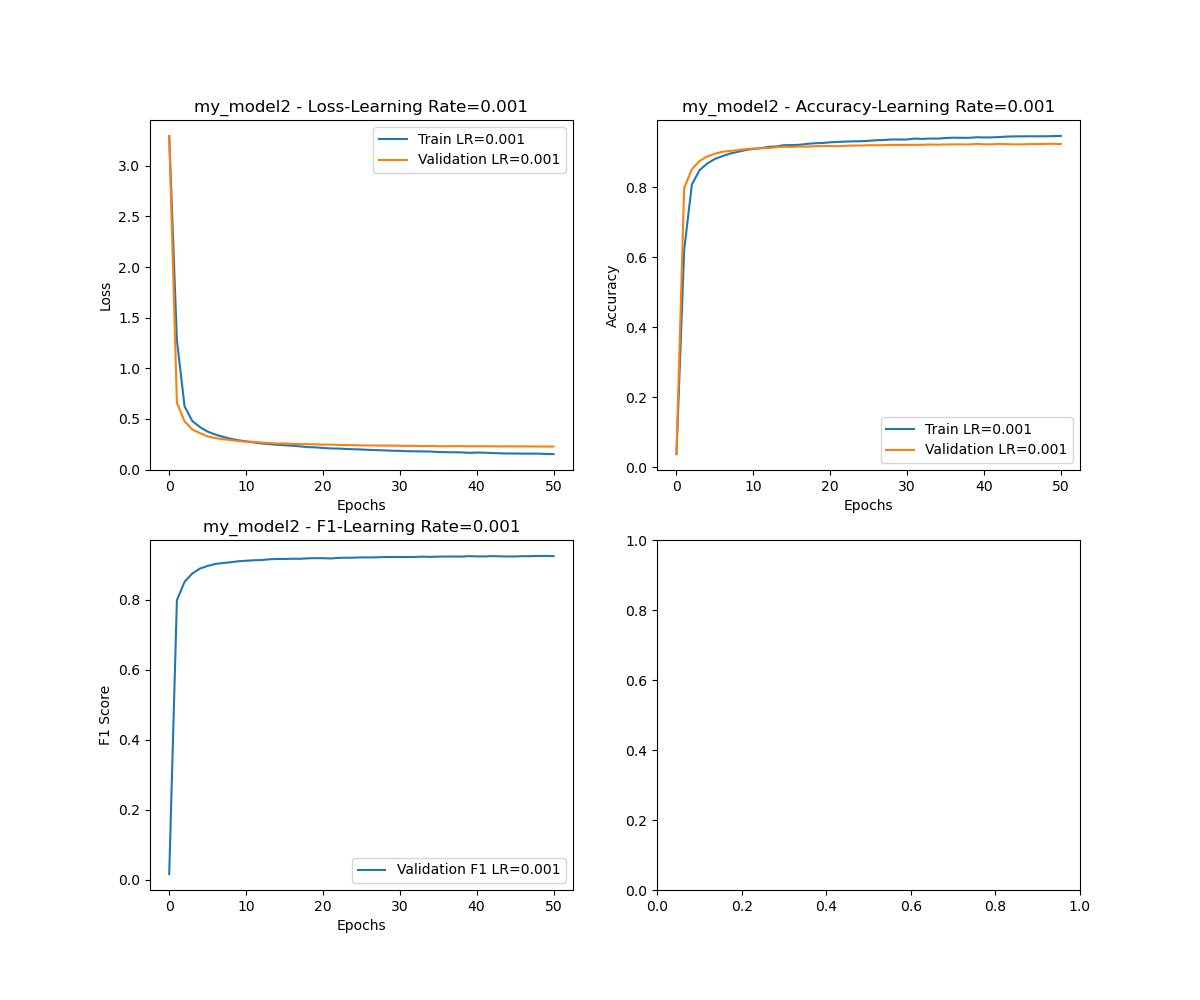
\includegraphics[width=\linewidth, height=6cm]{Images/my_model2_0.001.png} 
        \caption{Model 2 Learning Curve with Learning Rate 0.001}
        \label{fig:model2_lr_0.001}
    \end{subfigure}
    \begin{subfigure}{0.5\textwidth}
        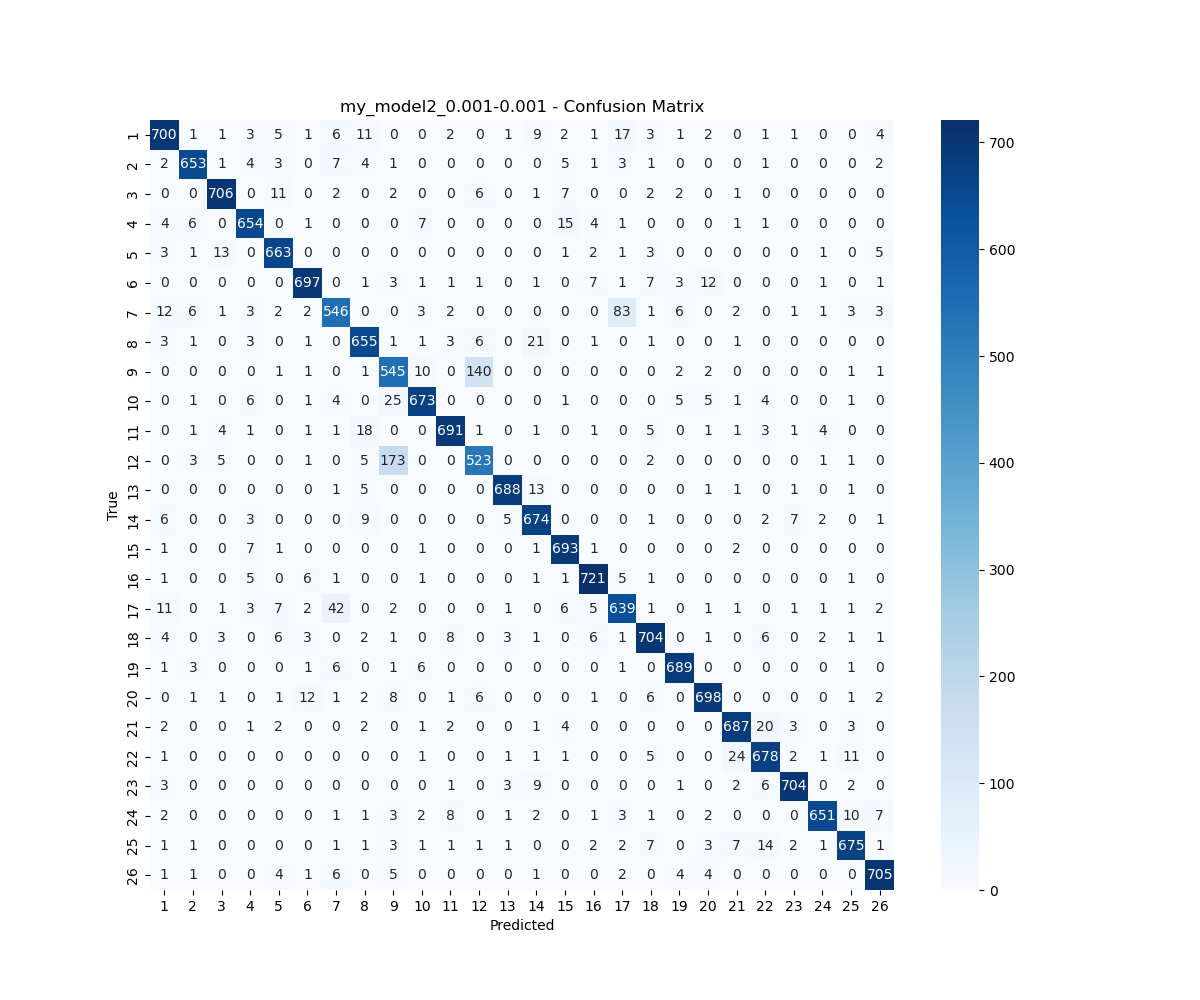
\includegraphics[width=\linewidth, height=6cm]{Images/my_model2_0.001-confusion_matrix} 
        \caption{Model 2 Confusion Matrix with Learning Rate 0.001}
        \label{fig:model2_lr_0.001_confusion_matrix}
    \end{subfigure}
    \caption{Model 2 Learning Curve and Confusion Matrix with Learning Rate 0.001}
    \label{fig:model2_lr_0.001_combined}
\end{figure}

\subsubsection{Learning Rate = 0.0005}
% Best epoch: 50, validation accuracy: 0.9159, validation f1 score: 0.9157, model name: my_model2_0.0005,
%           train loss: 0.2369, validation loss: 0.2604, train accuracy: 0.9225, validation accuracy: 0.9159
Best Performance:
\begin{itemize}
    \item Best epoch: 50
    \item train loss: 0.2369
    \item validation loss: 0.2604
    \item train accuracy: 0.9225
    \item validation accuracy: 0.9159
    \item validation f1 score: 0.9157
\end{itemize}

\begin{figure}[h]
    \begin{subfigure}{0.5\textwidth}
        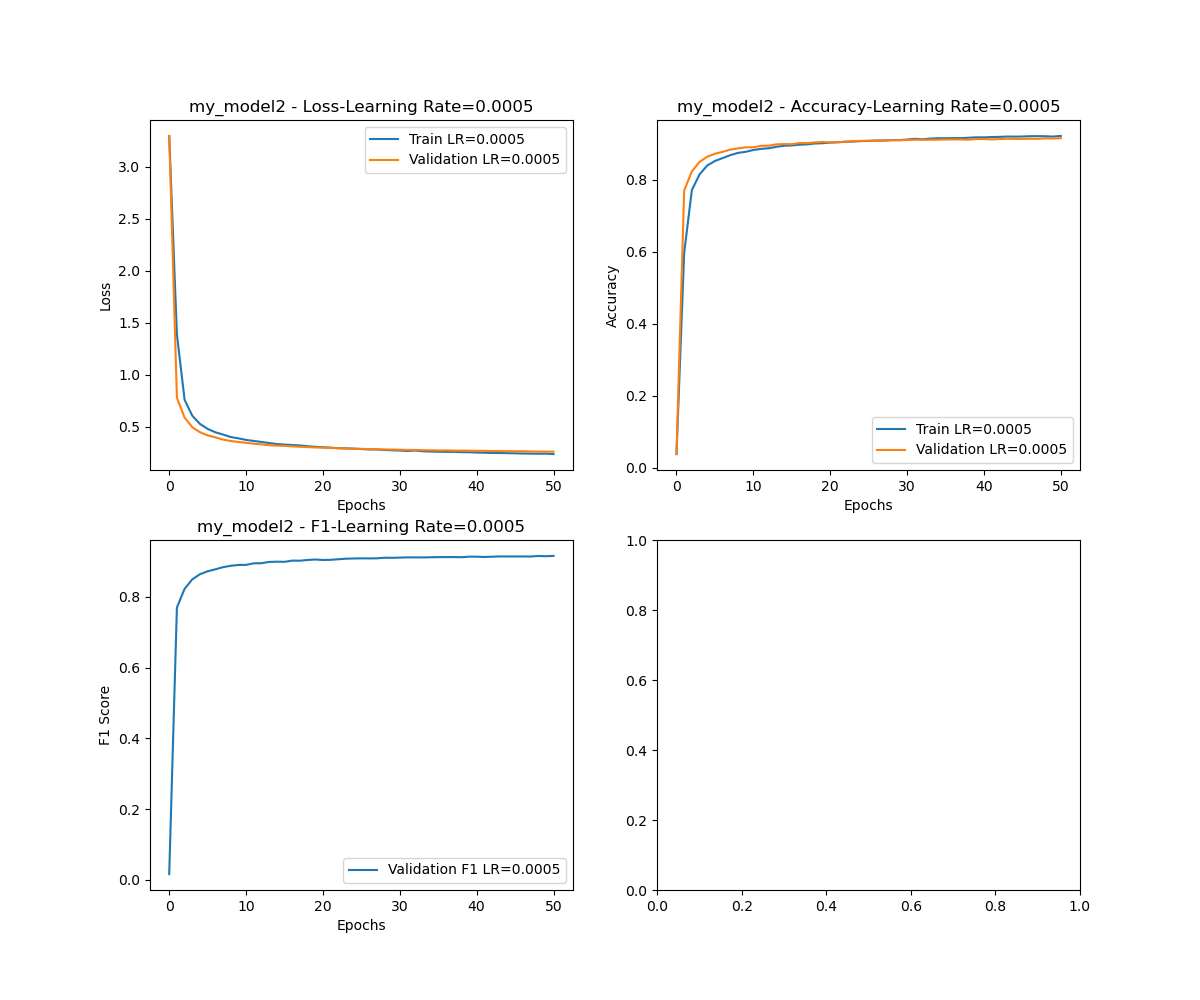
\includegraphics[width=\linewidth, height=6cm]{Images/my_model2_0.0005.png} 
        \caption{Model 2 Learning Curve with Learning Rate 0.0005}
        \label{fig:model2_lr_0.0005}
    \end{subfigure}
    \begin{subfigure}{0.5\textwidth}
        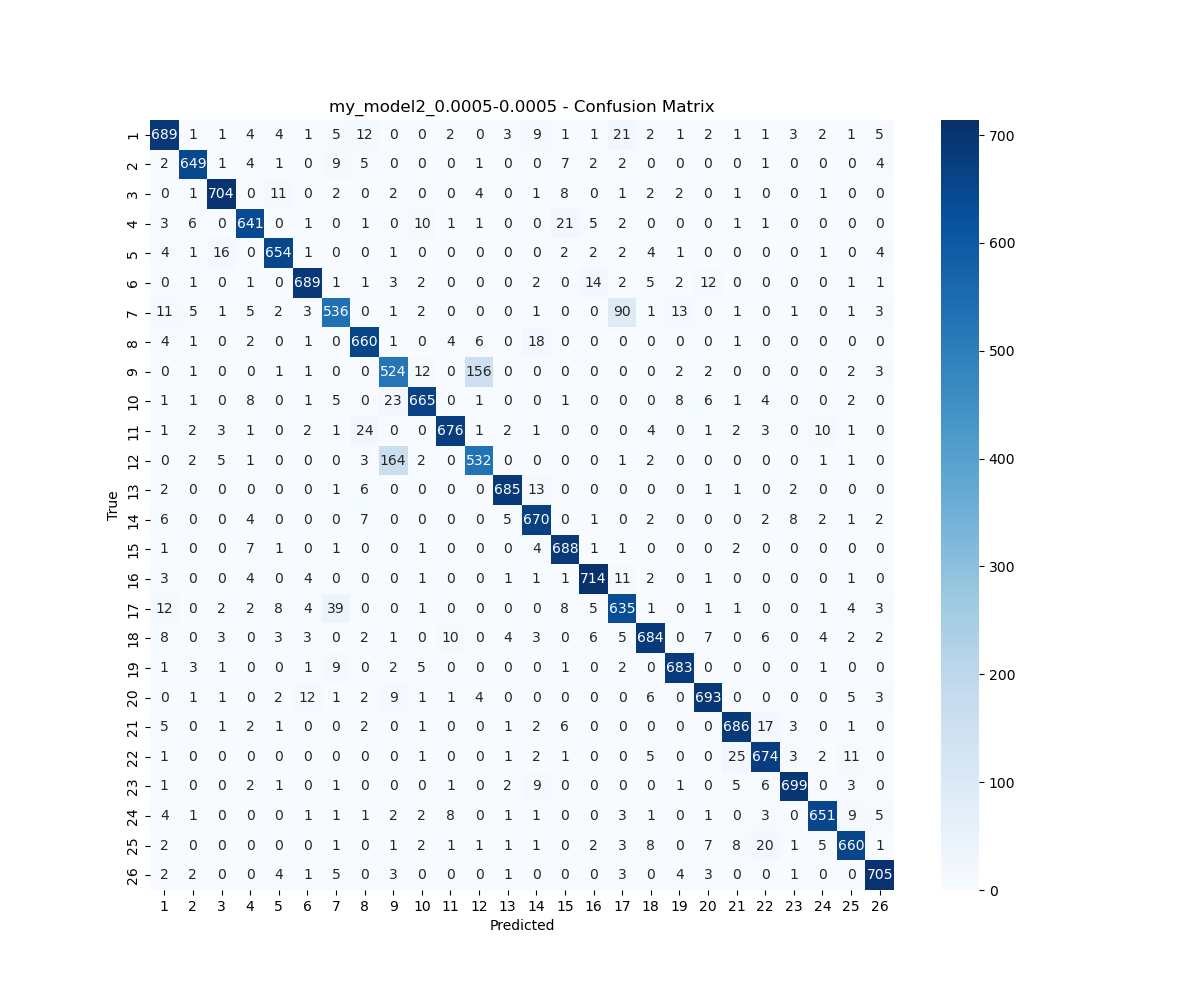
\includegraphics[width=\linewidth, height=6cm]{Images/my_model2_0.0005-confusion_matrix} 
        \caption{Model 2 Confusion Matrix with Learning Rate 0.0005}
        \label{fig:model2_lr_0.0005_confusion_matrix}
    \end{subfigure}
    \caption{Model 2 Learning Curve and Confusion Matrix with Learning Rate 0.0005}
    \label{fig:model2_lr_0.0005_combined}
\end{figure}

\subsection{Model 3}
\subsubsection{Architecture}
\begin{verbatim}
    Dense(784, 1024),
    Relu(),
    Dropout(probability=.2),
    Dense(1024, 512),
    Relu(),
    Dropout(probability=.2),
    Dense(512,26),
    Softmax()
\end{verbatim}

\subsubsection{Learning Rate = 0.01}
% Best epoch: 49, validation accuracy: 0.9161, validation f1 score: 0.9156, model name: my_model3_0.01,
%           train loss: 0.1794, validation loss: 0.2574, train accuracy: 0.9346, validation accuracy: 0.9161
Best Performance:
\begin{itemize}
    \item Best epoch: 49
    \item train loss: 0.1794
    \item validation loss: 0.2574
    \item train accuracy: 0.9346
    \item validation accuracy: 0.9161
    \item validation f1 score: 0.9156
\end{itemize}

\begin{figure}[h]
    \begin{subfigure}{0.5\textwidth}
        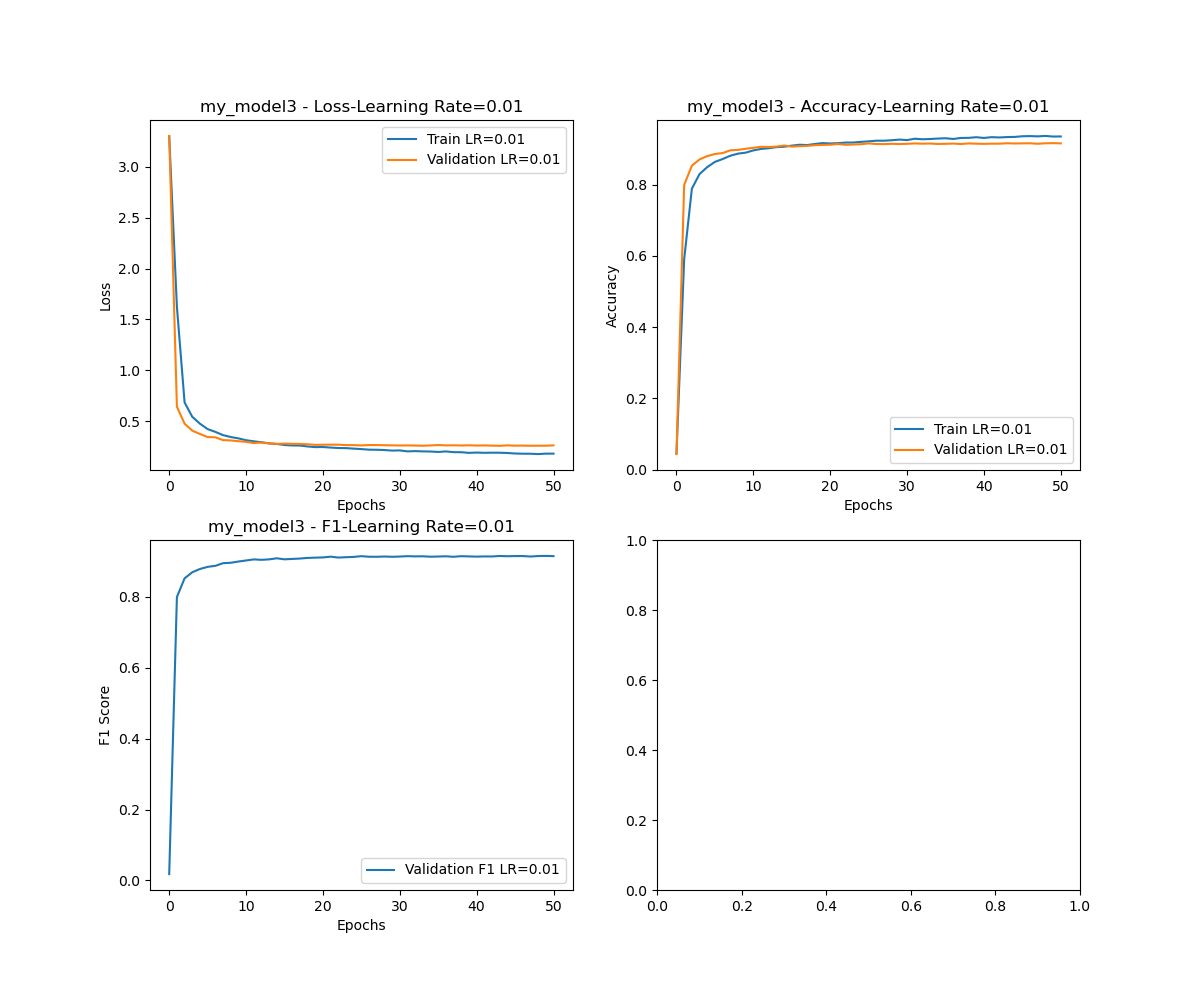
\includegraphics[width=\linewidth, height=6cm]{Images/my_model3_0.01.png} 
        \caption{Model 3 Learning Curve with Learning Rate 0.01}
        \label{fig:model3_lr_0.01}
    \end{subfigure}
    \begin{subfigure}{0.5\textwidth}
        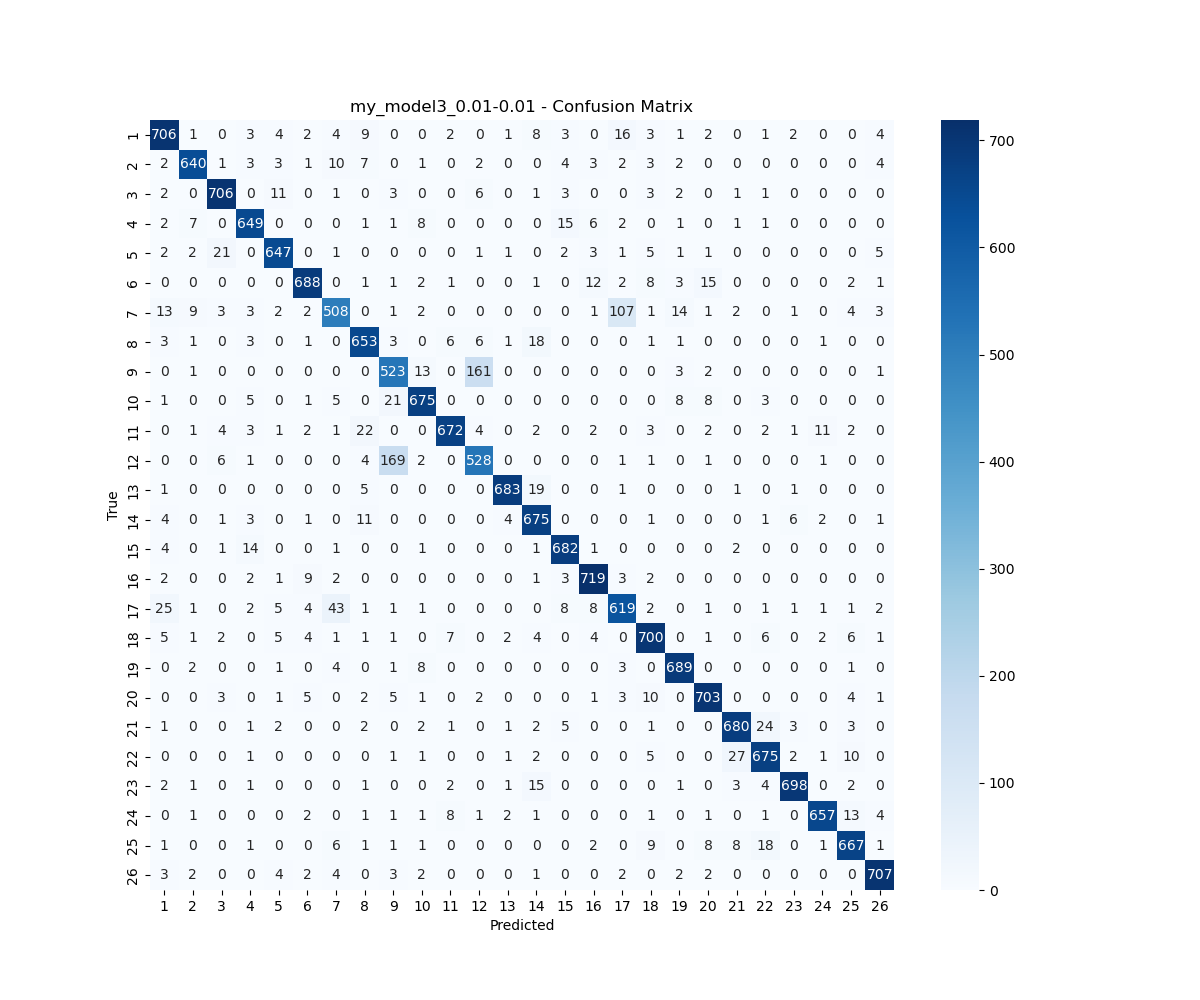
\includegraphics[width=\linewidth, height=5cm]{Images/my_model3_0.01-confusion_matrix} 
        \caption{Model 3 Confusion Matrix with Learning Rate 0.01}
        \label{fig:model3_lr_0.01_confusion_matrix}
    \end{subfigure}
    \caption{Model 3 Learning Curve and Confusion Matrix with Learning Rate 0.01}
    \label{fig:model3_lr_0.01_combined}
\end{figure}

\subsubsection{Learning Rate = 0.005}
% Best epoch: 35, validation accuracy: 0.9260, validation f1 score: 0.9257, model name: my_model3_0.005,
%           train loss: 0.1056, validation loss: 0.2440, train accuracy: 0.9599, validation accuracy: 0.9260
Best Performance:
\begin{itemize}
    \item Best epoch: 35
    \item train loss: 0.1056
    \item validation loss: 0.2440
    \item train accuracy: 0.9599
    \item validation accuracy: 0.9260
    \item validation f1 score: 0.9257
\end{itemize}

\begin{figure}[h]
    \begin{subfigure}{0.5\textwidth}
        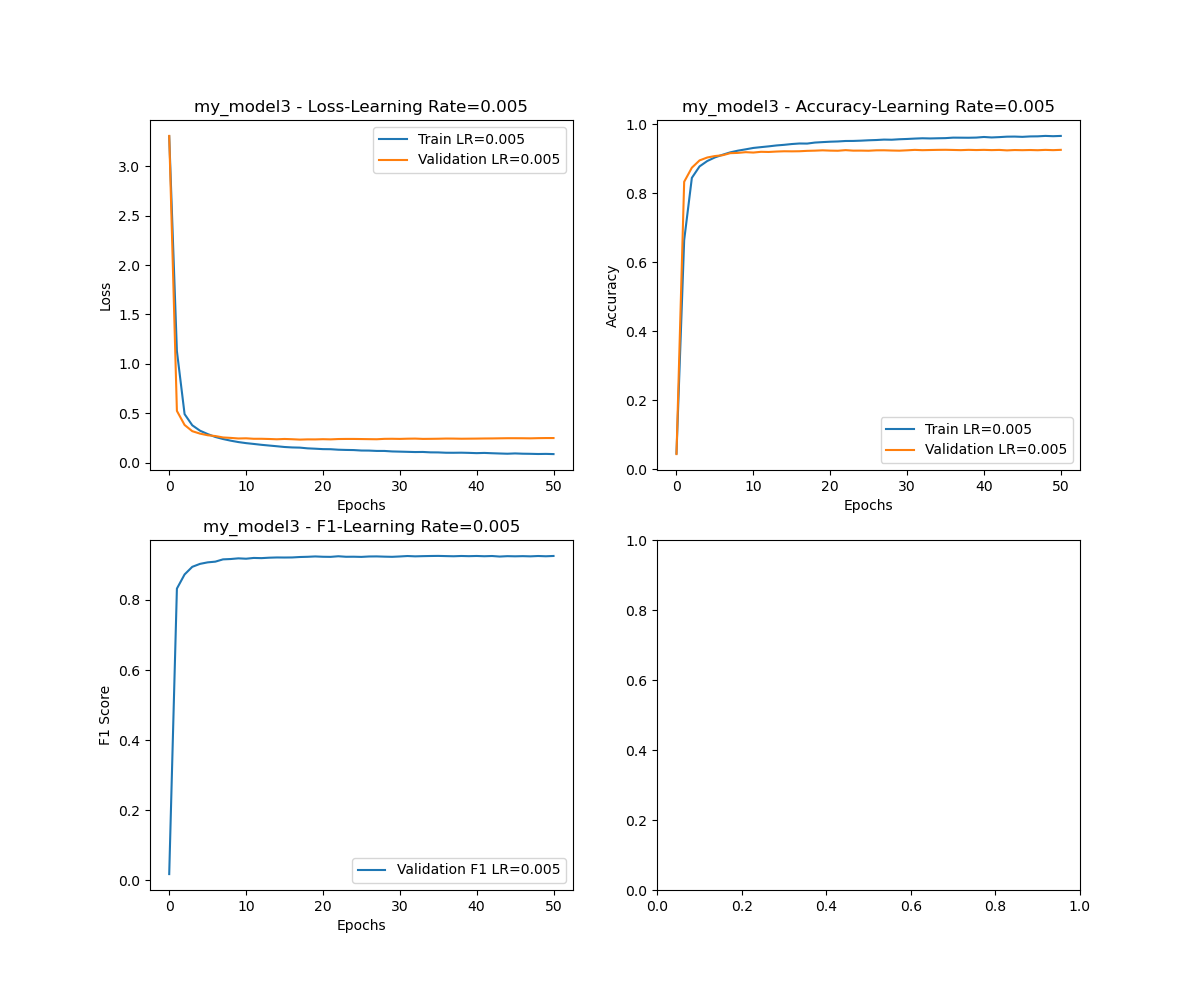
\includegraphics[width=\linewidth, height=5cm]{Images/my_model3_0.005.png} 
        \caption{Model 3 Learning Curve with Learning Rate 0.005}
        \label{fig:model3_lr_0.005}
    \end{subfigure}
    \begin{subfigure}{0.5\textwidth}
        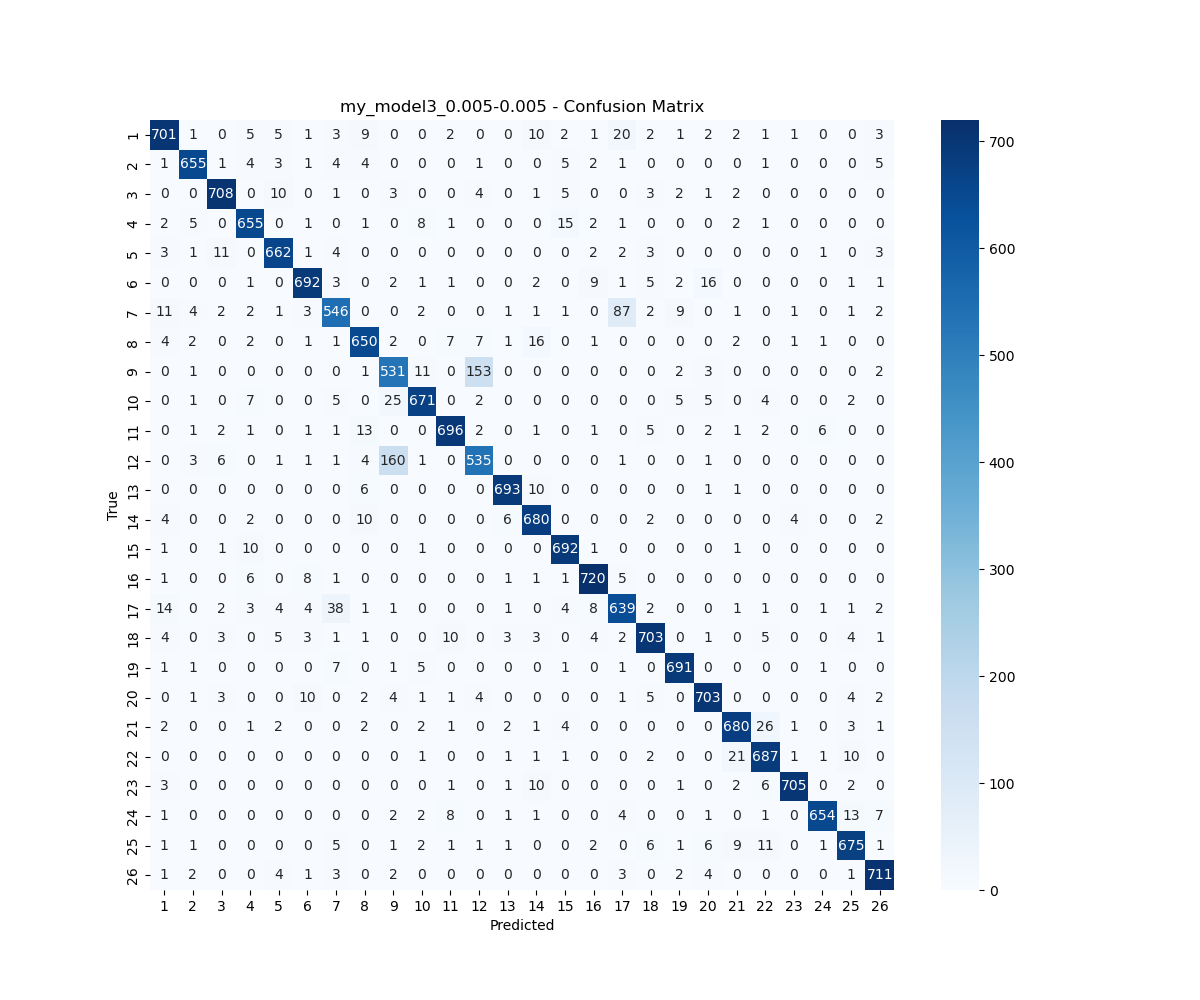
\includegraphics[width=\linewidth, height=5cm]{Images/my_model3_0.005-confusion_matrix} 
        \caption{Model 3 Confusion Matrix with Learning Rate 0.005}
        \label{fig:model3_lr_0.005_confusion_matrix}
    \end{subfigure}
    \caption{Model 3 Learning Curve and Confusion Matrix with Learning Rate 0.005}
    \label{fig:model3_lr_0.005_combined}
\end{figure}

\subsubsection{Learning Rate = 0.001}
% Best epoch: 41, validation accuracy: 0.9208, validation f1 score: 0.9205, model name: my_model3_0.001,
%           train loss: 0.1883, validation loss: 0.2434, train accuracy: 0.9366, validation accuracy: 0.9208
Best Performance:
\begin{itemize}
    \item Best epoch: 41
    \item train loss: 0.1883
    \item validation loss: 0.2434
    \item train accuracy: 0.9366
    \item validation accuracy: 0.9208
    \item validation f1 score: 0.9205
\end{itemize}

\begin{figure}[h]
    \begin{subfigure}{0.5\textwidth}
        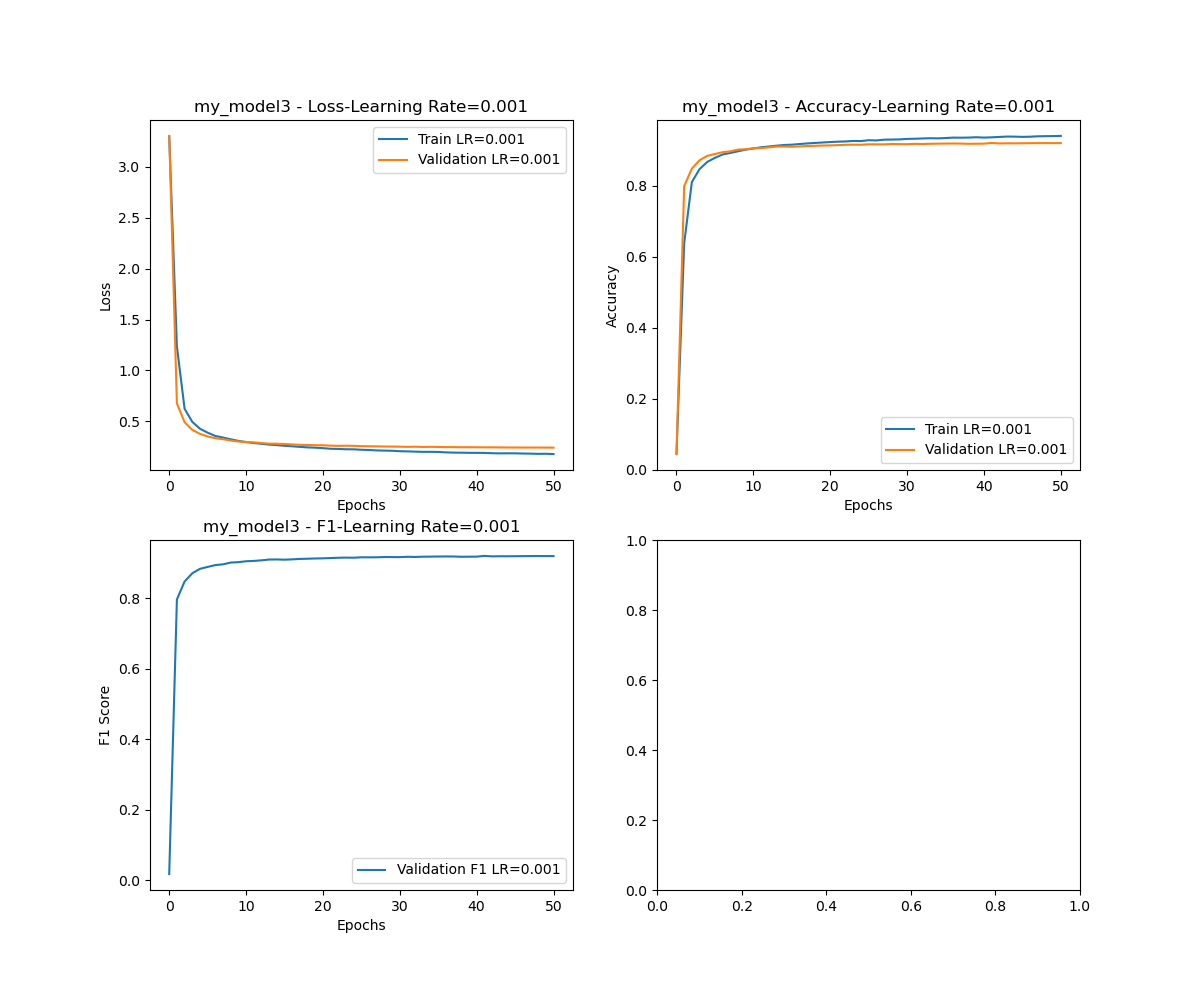
\includegraphics[width=\linewidth, height=5cm]{Images/my_model3_0.001.png} 
        \caption{Model 3 Learning Curve with Learning Rate 0.001}
        \label{fig:model3_lr_0.001}
    \end{subfigure}
    \begin{subfigure}{0.5\textwidth}
        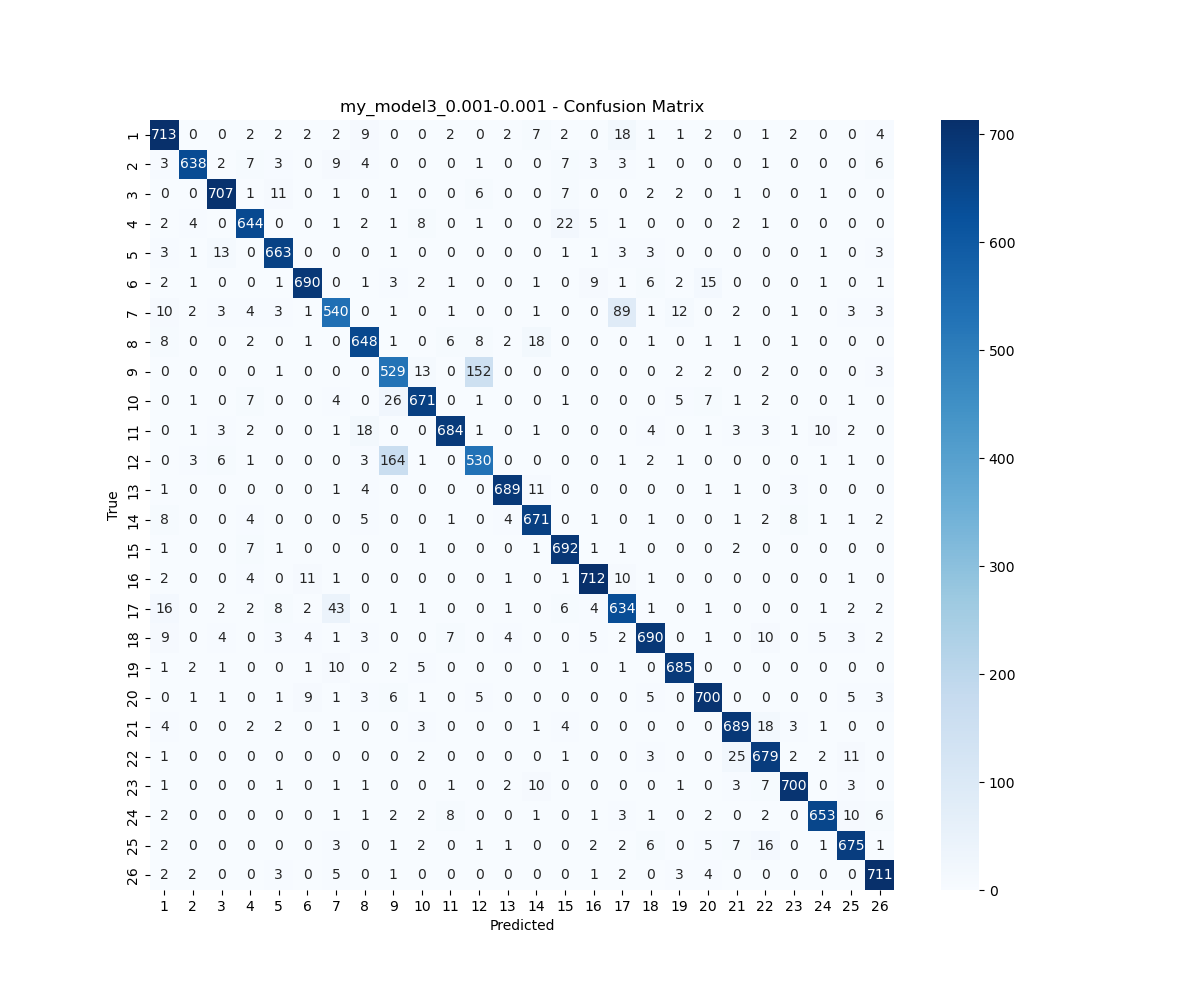
\includegraphics[width=\linewidth, height=5cm]{Images/my_model3_0.001-confusion_matrix} 
        \caption{Model 3 Confusion Matrix with Learning Rate 0.001}
        \label{fig:model3_lr_0.001_confusion_matrix}
    \end{subfigure}
    \caption{Model 3 Learning Curve and Confusion Matrix with Learning Rate 0.001}
    \label{fig:model3_lr_0.001_combined}
\end{figure}

\subsubsection{Learning Rate = 0.0005}
% Best epoch: 50, validation accuracy: 0.9074, validation f1 score: 0.9070, model name: my_model3_0.0005,
%           train loss: 0.2819, validation loss: 0.2898, train accuracy: 0.9101, validation accuracy: 0.9074
Best Performance:
\begin{itemize}
    \item Best epoch: 50
    \item train loss: 0.2819
    \item validation loss: 0.2898
    \item train accuracy: 0.9101
    \item validation accuracy: 0.9074
    \item validation f1 score: 0.9070
\end{itemize}

\begin{figure}[h]
    \begin{subfigure}{0.5\textwidth}
        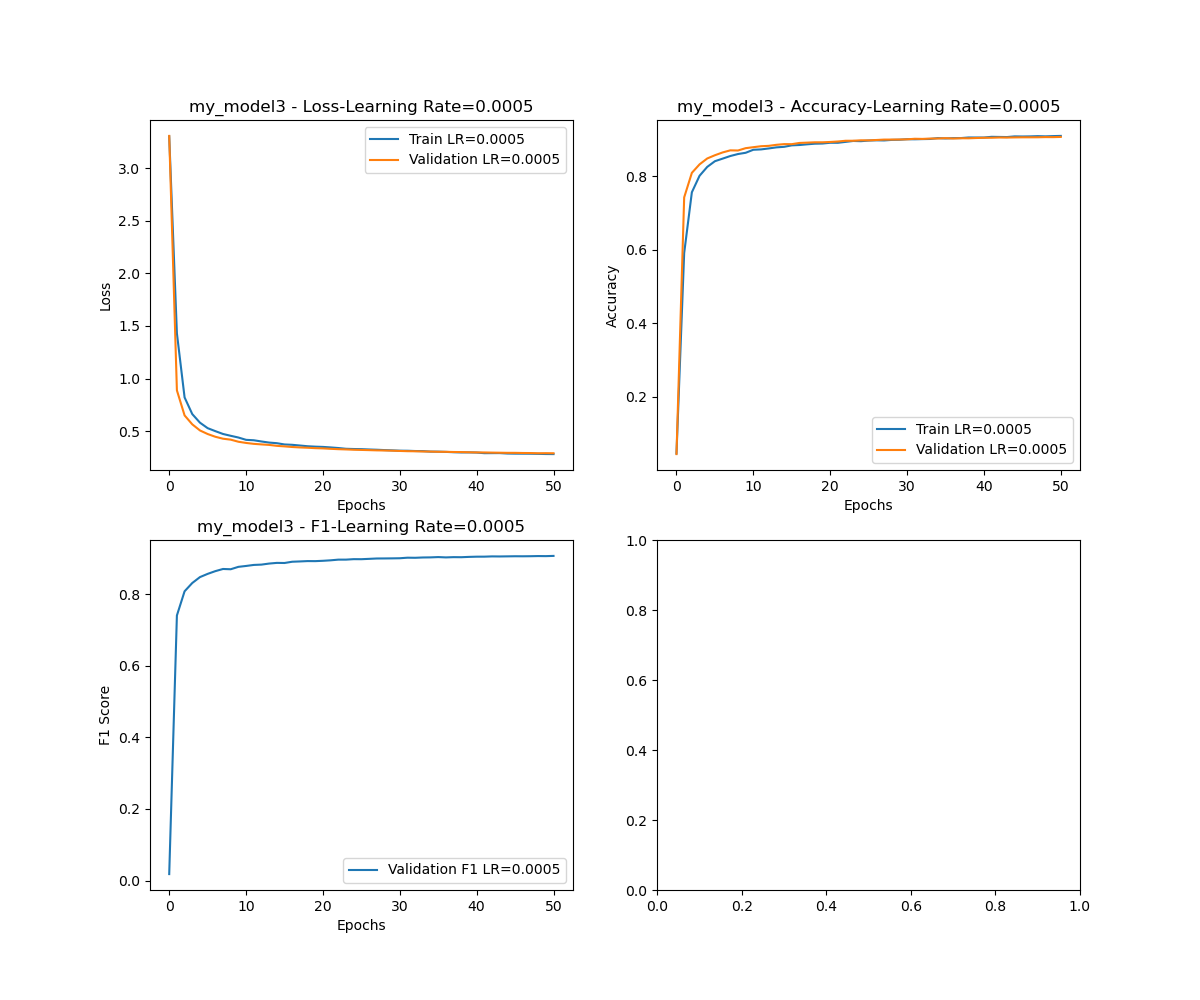
\includegraphics[width=\linewidth, height=5cm]{Images/my_model3_0.0005.png} 
        \caption{Model 3 Learning Curve with Learning Rate 0.0005}
        \label{fig:model3_lr_0.0005}
    \end{subfigure}
    \begin{subfigure}{0.5\textwidth}
        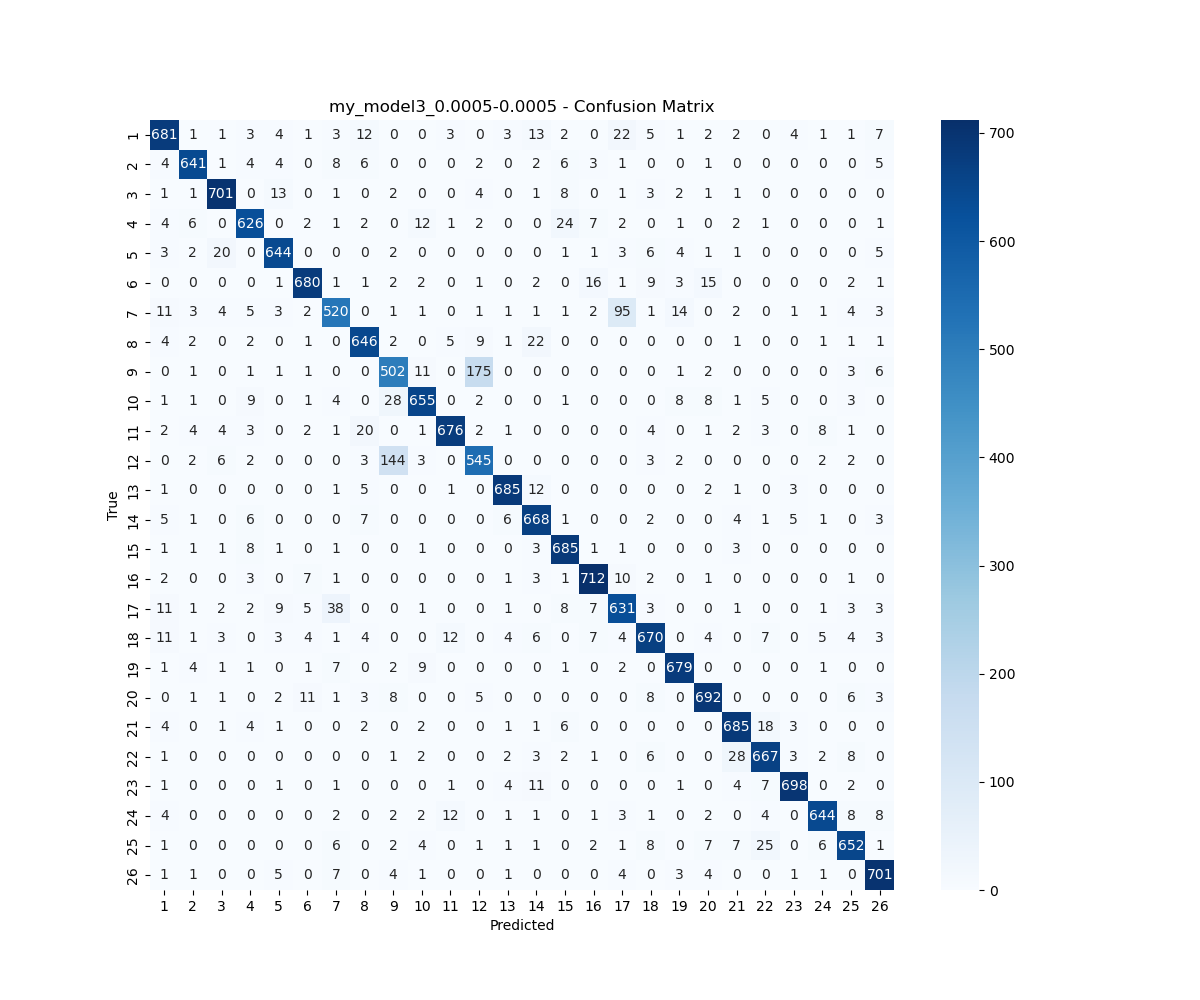
\includegraphics[width=\linewidth, height=5cm]{Images/my_model3_0.0005-confusion_matrix} 
        \caption{Model 3 Confusion Matrix with Learning Rate 0.0005}
        \label{fig:model3_lr_0.0005_confusion_matrix}
    \end{subfigure}
    \caption{Model 3 Learning Curve and Confusion Matrix with Learning Rate 0.0005}
    \label{fig:model3_lr_0.0005_combined}
\end{figure}

\section{Best Model}
\subsection{Model Architecture}
\begin{verbatim}
    Dense(784, 1024),
    Relu(),
    Dropout(probability=.2),
    Dense(1024, 512),
    Relu(),
    Dropout(probability=.2),
    Dense(512,26),
    Softmax()
\end{verbatim}
\subsection{Learning Rate}
\textbf{Learning Rate = 0.005}
\subsection{Performance on validation set}
Best Performance:
\begin{itemize}
    \item Best epoch: 50
    \item train loss: 0.0936
    \item validation loss: 0.2478
    \item train accuracy: 0.9647
    \item validation accuracy: 0.9268
    \item validation f1 score: 0.9265
\end{itemize}

\begin{figure}[h]
    \begin{subfigure}{0.5\textwidth}
        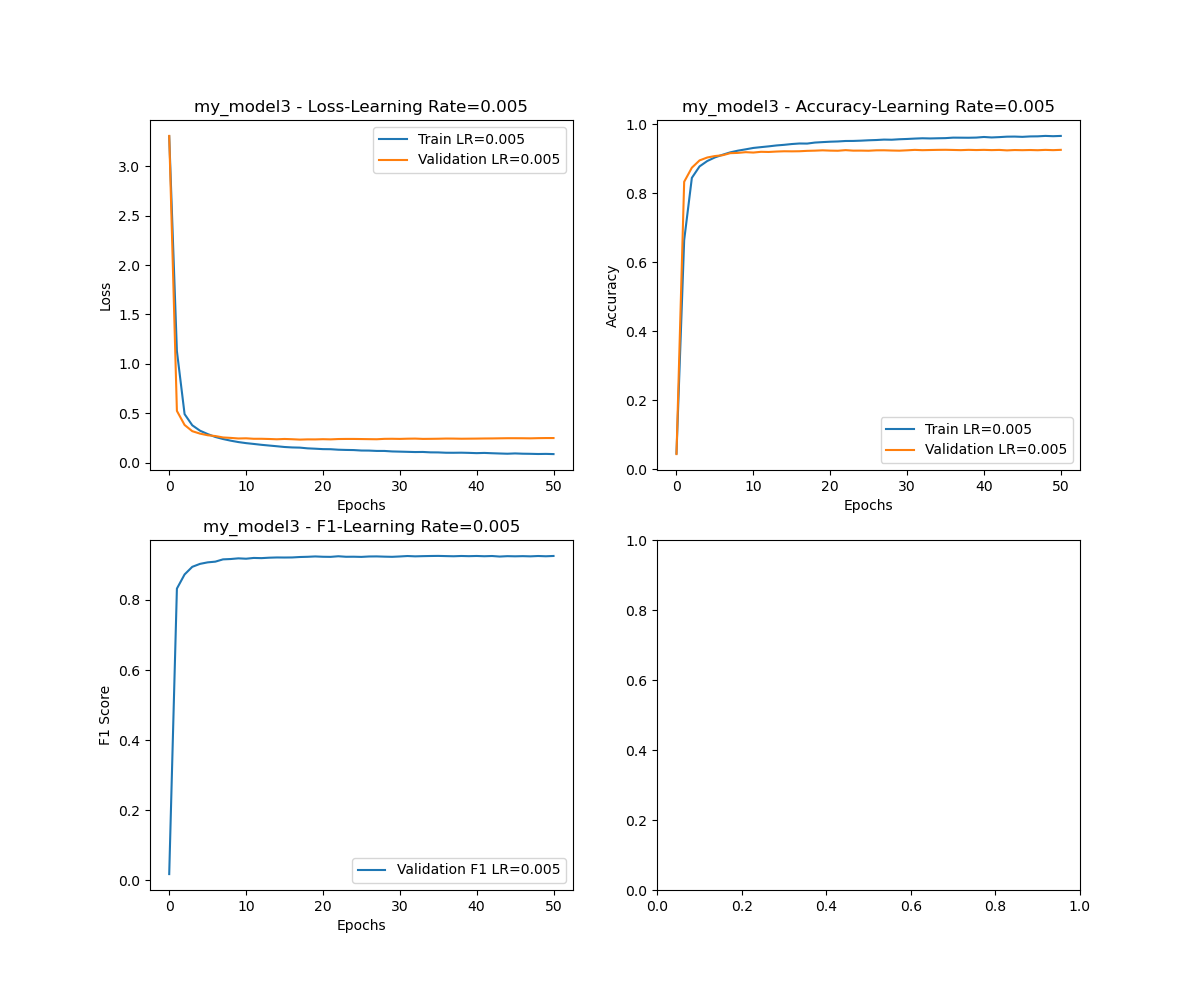
\includegraphics[width=\linewidth, height=5cm]{Images/my_model3_0.005.png} 
        \caption{Choosen Best Model Learning Curve}
        \label{fig:model3_lr_0.005_best}
    \end{subfigure}
    \begin{subfigure}{0.5\textwidth}
        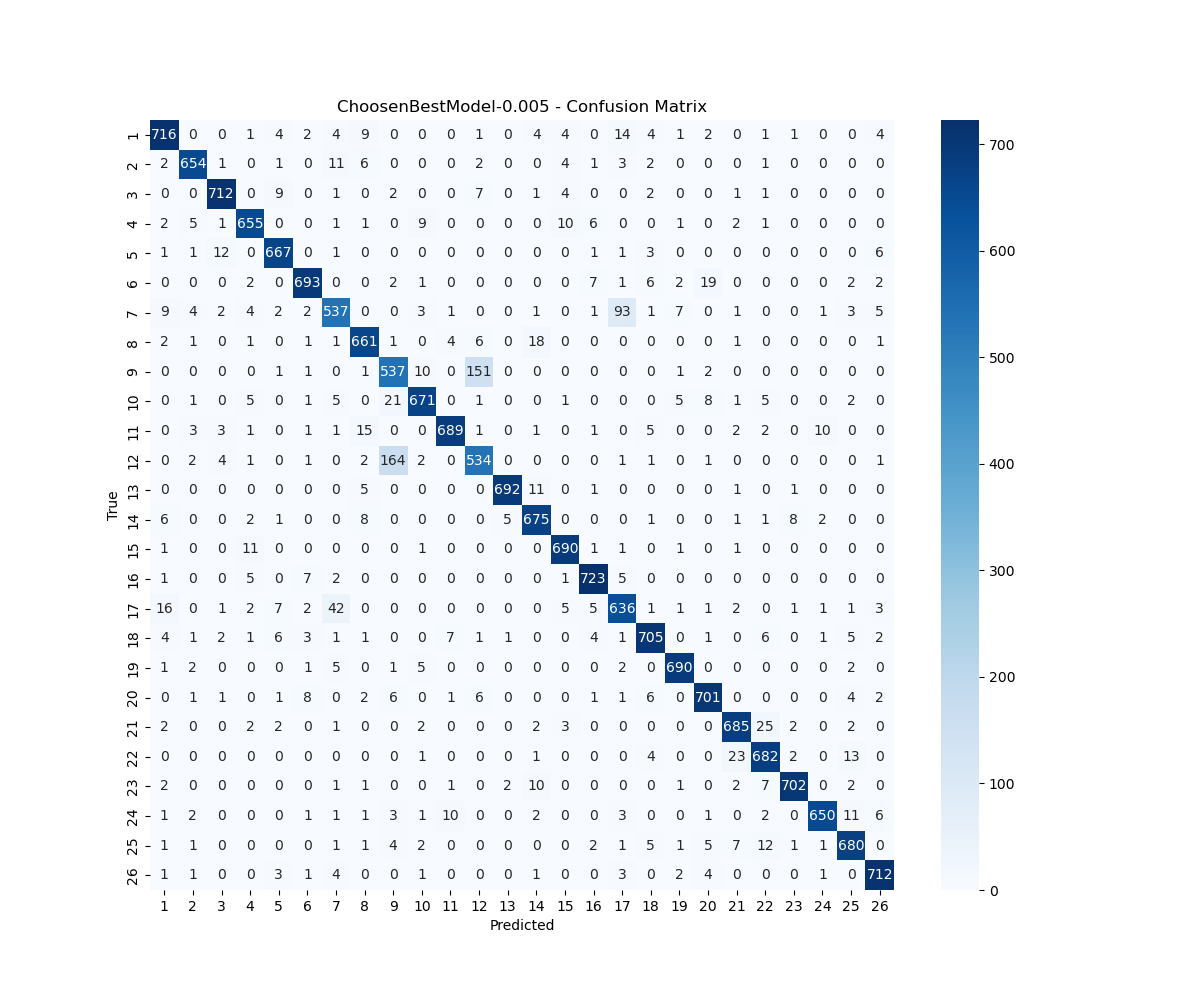
\includegraphics[width=\linewidth, height=5cm]{Images/ChoosenBestModel-confusion_matrix.png} 
        \caption{Choosen Best Model Confusion Matrix}
        \label{fig:model3_lr_0.005_confusion_matrix_best}
    \end{subfigure}
    \caption{Choosen Best Model Learning Curve and Confusion Matrix}
    \label{fig:model3_lr_0.005_combined_best}
\end{figure}

\section{Performance on Test Set}
% Test Loss:  0.26707993365492666
% Test Accuracy:  0.9237019230769231
% Test Macro F1 Score:  0.9237425799805024
\begin{itemize}
    \item Test Loss:  0.26707993365492666
    \item Test Accuracy:  0.9237019230769231
    \item Test Macro F1 Score:  0.9237425799805024
\end{itemize}
\begin{figure}[h]
    \centering
    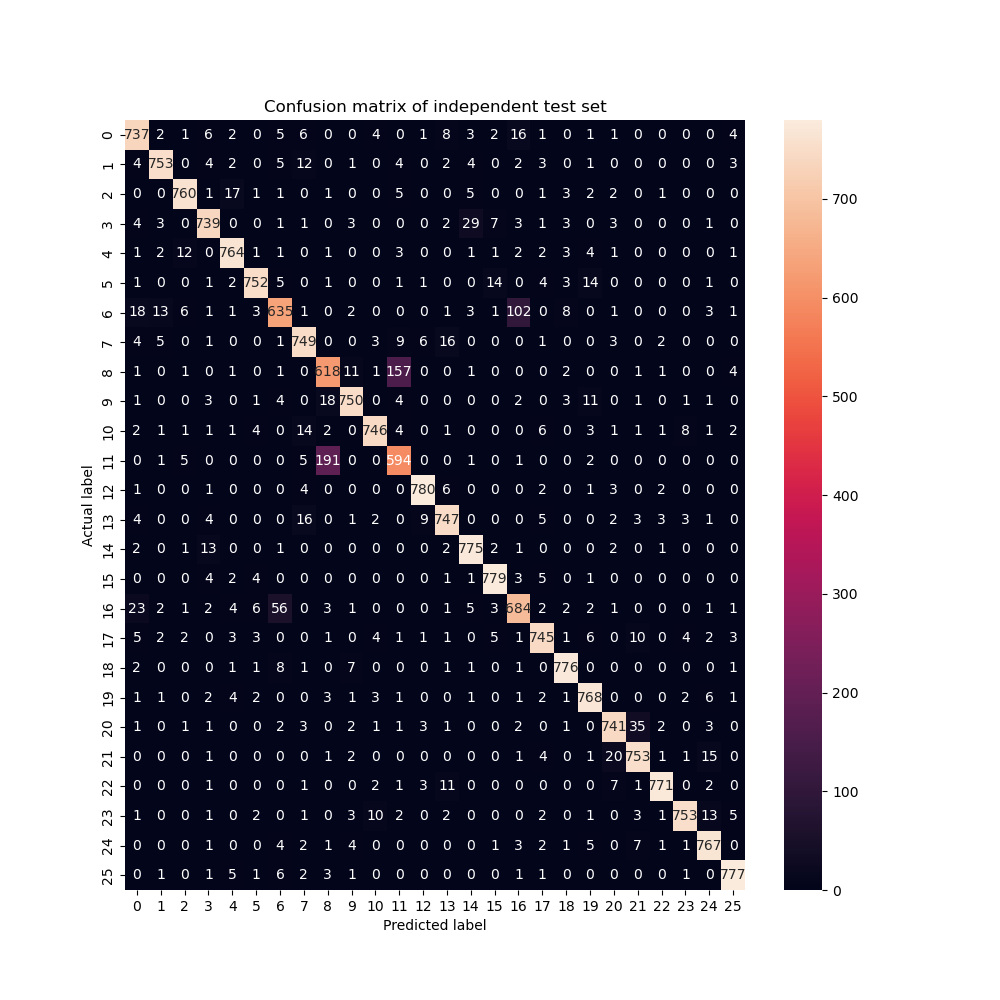
\includegraphics[width=0.5\linewidth]{Images/independent_test_set_confusion_matrix.png} 
    \caption{Choosen Best Model Confusion Matrix on Test Set}
    \label{fig:model3_lr_0.005_confusion_matrix_test}
\end{figure}
\end{document}
